\chapter{Teorie míry a dimenze}\label{chapter:teorie-miry-a-dimenze}

V této kapitole se budeme nyní věnovat fraktálům a jim příbuzným záležitostem trochu formálněji. Do této chvíle jsme si již stihli představit některé základní fraktály,~jako je např. \emph{Sierpińského trojúhelník},~\emph{Kochova vločka} nebo \emph{Cantorovo diskontinuum},~na nichž jsme si ilustrovali především myšlenku soběpodobnosti a na to navazující pojetí dimenze (viz kapitola \ref{chapter:uvod_do_fraktalu},~sekce \ref{sec:sobepodobnost} a \ref{sec:fraktalni_dimenze}).

Ačkoliv leckterý čtenář by se s~poskytnutým vysvětlením jistě spokojil,~jiný by mohl namítat,~že jsme řadu věcí vynechali. A měl by jistě pravdu. Proto se v~této kapitole budeme věnovat některým záležitostem z~tzv. \emph{teorie míry}\index{teorie míry},~která je v~tomto ohledu klíčová a poskytne nám nástroje pro měření fraktálních útvarů,~jejichž geometrie často přesahuje možnosti klasické "eukleidovské analýzy". \emph{Míra} pro nás představuje zobecnění pojmů jako je \emph{délka,~obsah} a \emph{objem},~které známe ze školní geometrie. Na jejím základě pak budeme schopni detailněji prozkoumat fraktální dimenzi,~kterou jsme již v~základu pokryli v~předešlé kapitole. Jmenovitě se budeme zabývat
\begin{itemize}
    \item \emph{měřitelnými prostory}\index{měřitelný prostor} a \emph{prostory s~mírou}\index{prostor s~mírou} obecně,
    \item \emph{lebesgueovou mírou}\index{Lebesgueova míra},
    \item \emph{box-counting dimenzí}\index{box-counting dimenze}\footnote{Též ji lze nalézt pod~názvem \emph{Minkowského dimenze}\index{Minkowského dimenze} nebo \emph{Minkowského-Bouligandova dimenze}\index{Minkowského-Bouligandova dimenze}. Je pojmenována po polském matematikovi \name{Hermannovi Minkowském} (1864--1909) a francouzském matematikovi \name{Georgesovi Bouligandovi} (1889--1979).}
    \item \emph{Hausdorffovou mírou} a z~ní vycházející \emph{Hausdorffovou dimenzí}.
\end{itemize}

Ačkoliv je toto téma jinak velice obsáhlé jsou mu věnované samostatné texty i~knihy,~spokojíme se pouze s~naprostým základem. Pro další znalosti si dovolím čtenáře odkázat na knihy \cite{Falconer2014},~\cite{Lukes2013},~\cite{NetukaIntegral2016} a~\cite{Edgar2008}.

Než se však pustíme do samotné problematiky,~je důležité zmínit,~že pro rigorózní budování budeme potřebovat některé základní znalosti. V~dalším textu předpokladáme,~že je s~nimi čtenář obeznámen. I~přesto si zde dovolíme začít soupisem pojmů a značení,~které budeme dále potřebovat. Některé záležitosti využijeme ještě v~kapitole \ref{chapter:hausdorffuv-mp} o~Hausdorffově metrickém prostoru.

\section{Základní pojmy a značení}\label{sec:zakladni-pojmy-a-znaceni}

V tomto oddílu se v~krátkosti zaměříme na připomenutí některých pojmů a značení,~které budeme dále využívat. Související teorii týkající se mnoha záležitostí v~tomto případě vynecháme s~předpokladem,~že ji čtenář již zná. Pokud tomu však v~některých případech takto nebude,~lze tuto část textu považovat za výčet konceptů,~které pro zvládnutí nadcházející teorie budeme potřebovat.

\todo{Doplnit pojmy a značení podle dalšího textu
    \begin{itemize}
        \item Limita funkce
        \item Limes superior/inferior
        \item Metrický prostor, úplný MP
        \item Cauchyovská posloupnost
        \item vzdálenost bodu od množiny
        \item Otevřená/uzavřená koule
        \item Otevřená/uzavřená množina
        \item Kompaktní množina, věta o kompaktnosti v $\R^n$, věta o uzavřenosti kompaktní množiny.
        \item Kvádr a objem kvádru
        \item Průměr množiny
        \item $\delta$-okolí množiny
        \item Pokrytí, zjemnění
        \item $\delta$-pokrytí
        \item $\delta$-mříž
        \item Vnitřek, hranice množiny
        \item (bi-)lipschitzovské zobrazení
    \end{itemize}
}
\section{Prostory s~mírou}\label{sec:prostory-s-mirou}

Jak již bylo zmíněno v~úvodu,~klíčovým pojmem v~této kapitole (a pro studium fraktálů obecně) je takzvaná \emph{míra}. Ta pro nás představuje obecný způsob,~jak můžeme množinám přiřadit v~jistém smyslu "velikost". Konkrétněji,~byť vágně,~lze říci,~že sestává-li množina z~konečného nebo spočetného množství "rozumných" částí,~pak součet velikostí všech těchto dílčích množin je roven velikosti celé množiny,~kterou nazveme její \emph{mírou}. Pro začátek celkem jednoduchá myšlenka.

Pro formální zavedení tohoto pojmu však budeme muset nejprve zavést ještě jiný pojem,~a to tzv. \emph{$\sigma$-algebru}.

\subsection{Měřitelné prostory}\label{subsec:meritelne-prostory}

\begin{definition}[$\sigma$-algebra]\label{def:sigma-algebra}
    Nechť je dána libovolná množina $X$ a systém podmnožin $\mathcal{A}\subseteq\powset{X}$. Pak $\mathcal{A}$ je \emph{$\sigma$-algebra}\index{$\sigma$-algebra} na množině $X$,~pokud:
    \begin{enumerate}[label=(\alph*)]
        \item\label{def:sigma-algebra-podm1} $X\in\mathcal{A}$.
        \item\label{def:sigma-algebra-podm2} Pro každou množinu $A\in\mathcal{A}$ platí $X\setminus A\in\mathcal{A}$.
        \item\label{def:sigma-algebra-podm3} Pro libovolné množiny $A_1,A_2,\ldots\in\mathcal{A}$ platí $\bigcup_{i=1}^\infty A_i\in\mathcal{A}$.
    \end{enumerate}
    Dvojice $(X,\mathcal{A})$ se nazývá měřitelný prostor\index{prostor!měřitelný}.
\end{definition}

\begin{example}
    Jednoduché příklady $\sigma$-algeber:
    \begin{itemize}
        \item Triviálními příklady $\sigma$-algeber jsou množiny $\emptyset$,~$\powset{X}$ a~$\set{\emptyset,X}$ pro libovolnou množinu $X$.
        \item Pro konečnou množinu $X=\set{a,b,c,d}$ je jednou možnou $\sigma$-algebrou systém množin
        \[\Sigma=\set{\emptyset,\set{a,b},\set{c,d},\set{a,b,c,d}}.\]
    \end{itemize}
    Sami se zkuste přesvědčit,~že všechny zmíněné příklady vyhovují definici \ref{def:sigma-algebra}.
\end{example}

Než vyslovíme něco dalšího o~$\sigma$-algebrách a jejich významu,~podíváme se na seznam některých vesměs jednoduchých pozorováních zformulovaných níže v~tvrzení \ref{thm:sigma-algebra-vlastnosti}.
\begin{theorem}[Vlastnosti $\sigma$-algebry]\label{thm:sigma-algebra-vlastnosti}
    Nechť $(X,\mathcal{A})$ je meřitelný prostor. Pak platí:
    \begin{enumerate}[label=(\roman*)]
        \item $\emptyset\in\mathcal{A}$.
        \item Pro libovolné množiny $A_1,A_2,\ldots\in\mathcal{A}$ platí $\bigcap_{i=1}^\infty A_i\in\mathcal{A}$.
        \item Pro všechny množiny $A_1,A_2,\ldots,A_n\in\mathcal{A}$ platí
        \[\bigcup_{i=1}^n A_i\in\mathcal{A}\land\bigcap_{i=1}^n A_i\in\mathcal{A}.\]
        \item Jsou-li $A,B\in\mathcal{A}$ pak $A\setminus B\in\mathcal{A}$.
    \end{enumerate}
\end{theorem}

Z tohoto tvrzení je již lépe vidět,~proč jsou pro nás $\sigma$-algebry tak příjemným objektem. Jsou totiž \emph{uzavřené} na všechny základní množinové operace. To se nám bude později hodit při zavedení míry,~ke které směřujeme. Důkaz těchto dílčích tvrzení přitom není nikterak složitý.
\begin{proof}
    Mějme $\sigma$-algebru $\mathcal{A}$ na množině $X$.
    \begin{enumerate}[label=\textit{(\roman*)}]
        \item Z~podmínky \ref{def:sigma-algebra-podm1} definice \ref{def:sigma-algebra} víme,~že $X\in\mathcal{A}$ a z~podmínky \ref{def:sigma-algebra-podm2} tedy plyne $X\setminus X=\emptyset\in\mathcal{A}$.
        \item Mějme množiny $A_1,A_2,\ldots\in\mathcal{A}$. Společně s~využitím De Morganových zákonů plyne následující:
        \[\bigcap\limits_{i=1}^\infty A_i=\overbrace{X\setminus\underbrace{\bigcup\limits_{i=1}^\infty \overbrace{(X\setminus A_i)}^{\text{$\in\mathcal{A}$ podle \ref{def:sigma-algebra-podm2}}}}_{\text{$\in\mathcal{A}$ podle \ref{def:sigma-algebra-podm3}}}}^\text{$\in\mathcal{A}$ podle \ref{def:sigma-algebra-podm2}}\in\mathcal{A}.\]
        \item Nechť jsou dány množiny $A_1,A_2,\ldots,A_n\in\mathcal{A}$. Když pro každé $j>n$ položíme $A_j=\emptyset$,~pak platí
        \[\bigcup\limits_{i=1}^n A_i=\bigcup\limits_{i=1}^\infty A_i\in\mathcal{A}\]
        a podobně pro $\bigcap_{i=1}^n A_i\in\mathcal{A}$ podle předešlého bodu.
        \item Pro libovolné množiny $A,B\in\mathcal{A}$ platí
        \[A\setminus B=\overbrace{A\cup\underbrace{(X\setminus B)}_{\text{$\in\mathcal{A}$ podle \ref{def:sigma-algebra-podm2}}}}^{\text{$\in\mathcal{A}$ podle \ref{def:sigma-algebra-podm3}}}\in\mathcal{A}.\]
    \end{enumerate}
\end{proof}

\subsection{Míra}\label{subsec:mira}

V tuto chvíli máme již vše potřebné k~zavedení pojmu míra,~resp. prostor s~mírou.
\begin{definition}[Prostor s~mírou]\label{def:prostor-s-mirou}
    Nechť $(X,\mathcal{A})$ je měřitelný prostor. Zobrazení $\mapping{\mu}{\mathcal{A}}{\langle0,\infty\rangle}$ se nazývá \emph{míra}\index{míra} na $\mathcal{A}$,~pokud platí:
    \begin{enumerate}[label=(\alph*)]
        \item\label{def:mira-podm1} $\mu(\emptyset)=0$,
        \item\label{def:mira-podm2} pro množiny $A_1,A_2,\ldots$, kde $A_i\in\mathcal{A}$ pro každé $i\in\N$, po dvou disjunktní je
        \[\mu\left(\bigcup\limits_{i=1}^\infty A_i\right)=\sum_{i=1}^\infty\mu(A_i).\mathrightnote{$\sigma$-aditivita}\]
    \end{enumerate}
    Uspořádanou trojici $(X,\mathcal{A},\mu)$ nazýváme \emph{prostor s~mírou}\index{prostor!s mírou}\index{prostor s~mírou}.
\end{definition}

Vzhledem k~tomu,~co míra reprezentuje (tj. zobecnění délky,~obsahu,~objemu),~jsou tyto požadavky intuitivně dosti smysluplné.

\begin{example}\label{ex:mira}
    Příklady prostorů s~mírou:
    \begin{itemize}
        \item Asi pro nás nejtypičtější způsob,~jak měřit "velikost" množiny,~je podle \emph{počtu prvků}. Pro libovolnou množinu $X$ a potenční množinu $\powset{X}$ lze definovat prostor s~mírou $(X,\powset{X},\mu)$,~kde pro libovolnou množinu $A\in\powset{X}$ položíme $\mu(A)=|A|$. Takto definované míře $\mu$ říkáme \emph{aritmetická míra}\index{míra!aritmetická}.
        \item Máme libovolnou množinu $X$ a $\sigma$-algebru $\mathcal{A}$. Zvolme si pevně $x\in X$. Míru libovolné množiny $A\in\mathcal{A}$ lze definovat jako $\delta_x(A)=\chi_A(x)$,~kde $\chi_A$ je charakteristická funkce množiny $A$. Zobrazení $\delta_x$ je tzv. \emph{Diracova míra}\index{míra!Diracova}.
        \item Zobrazení přiřazující náhodnému jevu pravděpodobnost je též případem míry. Označíme-li si $\Omega=\set{\omega_1,\omega_2,\ldots,\omega_n}$ množinu všech elementárních jevů a $\mathcal{F}\subseteq\powset{\Omega}$,~pak $\mapping{\mathsf{P}}{\mathcal{F}}{\langle0,1\rangle}$ definovaná pro $A\in\mathcal{F}$ jako
        \[\mathsf{P}(A)=\dfrac{|A|}{|\Omega|}\]
        je mírou na $\mathcal{F}$. Speciálně $\mathsf{P}(\Omega)=1$.
    \end{itemize}
\end{example}

Ve všech případech zobrazení $\mu$ v~příkladu \ref{ex:mira} se lze snadno přesvědčit,~že se jedná o~míru,~tedy že splňuje podmínky \ref{def:mira-podm1} a \ref{def:mira-podm2} uvedené v~definici \ref{def:prostor-s-mirou} výše.

Pojďme nyní prozkoumat vlastnosti míry trochu hlouběji.
\begin{theorem}[Vlastnosti míry]\label{thm:mira-vlastnosti}
    Nechť $\mu$ je míra na $\sigma$-algebře $\mathcal{A}$. Pak platí následující:
    \begin{enumerate}[label=(\roman*)]
        \item\label{thm:mira-aditivita} Jsou-li množiny $A_1,A_2,\ldots,A_n\in\mathcal{A}$ po dvou disjunktní,~pak
        \[\mu\left(\bigcup_{i=1}^n A_i\right)=\sum_{i=1}^{n}\mu(A_i).\mathrightnote{aditivita\index{aditivita}}\]
        \item\label{thm:mira-monotonie} Pokud $A,B\in\mathcal{A}$ a $A\subseteq B$,~pak
        \[\mu(A)\leqslant\mu(B).\mathrightnote{monotonie míry\index{monotonie míry}}\]
        Navíc pokud $\mu(A)<\infty$,~pak $\mu(B\setminus A)=\mu(B)-\mu(A)$.
        \item\label{thm:mira-nekl-posl} Pokud $A_1,A_2,\ldots$,~kde $A_i\in\mathcal{A}$ pro každé $i\in\N$,~je neklesající posloupnost množin\footnote{Posloupnost množin,~kde $A_i\subseteq A_{i+1}$ pro každé $i\in\N$.},~pak
        \[\lim_{j\to\infty}\mu(A_j)=\mu\left(\bigcup_{j=1}^\infty A_j\right).\]
        \item\label{thm:mira-nerost-posl} Pokud $A_1,A_2,\ldots$, kde $A_i\in\mathcal{A}$ pro každé $i\in\N$, je nerostoucí posloupnost množin\footnote{$A_i\supseteq  A_{i+1}$ pro každé $i\in\N$.} a~navíc $\mu(A_1)<\infty$,~pak
        \[\lim_{j\to\infty}\mu(A_j)=\mu\left(\bigcap_{j=1}^\infty A_j\right).\]
        \item\label{thm:mira-sigma-subaditivita} Pokud $A_1,A_2,\ldots$,~kde $A_i\in\mathcal{A}$ pro každé $i\in\N$,~pak
        \[\mu\left(\bigcup_{i=1}^\infty A_i\right)\leqslant\sum_{i=1}^{\infty}\mu(A_i).\mathrightnote{$\sigma$-subaditivita}\]
    \end{enumerate}
\end{theorem}

Poslední vlastnost \ref{thm:mira-sigma-subaditivita} je tzv. \emph{$\sigma$-subaditivita}\index{$\sigma$-subaditivita}\footnote{V matematické terminologii se předpona $\sigma$ běžně týká spočetných sjednocení. \citep[str. 2]{Lukes2013}}. Oproti $\sigma$-aditivitě\index{$\sigma$-aditivita} se liší tím,~že u~množin $A_1,A_2,\dots$ se nepožaduje,~aby byly po dvou disjunktní,~tzn. mohou se "překrývat". Je však intuitivně nejspíše jasné,~že součtem měr všech těchto množin určitě nemůžeme získat míru nižší než je míra jejich sjednocení (dané "překryvy" započítáváme v~sumě vícekrát). Podobně i~monotonie dává intuitivně smysl,~neboť část větší množiny jistě nemůže mít větší míru než celek. Na formální stránku věci se podíváme nyní.
\begin{proof}
    V~důkazu využijeme některé vlastnosti $\sigma$-algebry z~věty \ref{thm:sigma-algebra-vlastnosti},~zejména,~že všechny množiny níže jsou opět prvky $\sigma$-algebry~$\mathcal{A}$.
    \begin{enumerate}[label=\textit{(\roman*)}]
        \item Pokud pro každé $j>n$ položíme $A_j=\emptyset$,~pak z~definice míry plyne
        \[\mu\left(\bigcup_{i=1}^n A_i\right)=\mu\left(\bigcup_{i=1}^\infty A_i\right)=\sum_{i=1}^{\infty}\mu(A_i)=\sum_{i=1}^{n}\mu(A_i).\]
        \item Nechť jsou dány $A,B\in\mathcal{A}$,~takové,~že $A\subseteq B$. Pak $B=A\cup(B\setminus A)$,~přičemž $A$ a $B\setminus A$ jsou disjunktní. Tedy podle bodu \ref{def:mira-podm2} lze psát $\mu(B)=\mu(A)+\mu(B\setminus A)\geqslant\mu(A)$,~protože $\mu(B\setminus A)\geqslant 0$.
        \item Mějme neklesající posloupnost množin $A_1,A_2,\ldots$,~kde $A_i\in\mathcal{A}$ pro každé $i\in\N$ (viz obrázek \ref{fig:nekl-posl-mnozin}).
        Definujeme posloupnost\footnote{V podstatě konstruujeme množiny $A_1,A_2,\ldots$ tak,~aby v~následující množině $A_i$ nebyl obsažen prvek,~který se nachází již v~některé z~množin $A_1,A_2,\ldots,A_{i-1}$. Podobná myšlenka je využita i~při důkazu budů \ref{thm:mira-nerost-posl} a \ref{thm:mira-sigma-subaditivita}.} množin $B_1,B_2,\ldots$ následovně:
        \[B_1=A_1,\;B_2=A_2\setminus A_1,\;B_i=A_i\setminus A_{i-1},\;i\geqslant 2.\]
        Množiny $B_1,B_2,\dots$ jsou po dvou disjunktní a zároveň\\$\bigcup_{i=1}^\infty B_i=\bigcup_{i=1}^\infty A_i$. Libovolnou množinu $A_n$ lze totiž zapsat jako
        \[A_n=\bigcup_{i=1}^n (A_i\setminus A_{i-1})=\bigcup_{i=1}^n B_i.\] 
        Podle již dokázaného bodu \ref{thm:mira-aditivita} (aditivita míry) tedy pro každé $n$ platí $\mu(A_n)=\sum_{i=1}^{n}\mu(B_i)$.
        Celkově
        \[\mu\left(\bigcup_{i=1}^\infty A_i\right)=\mu\left(\bigcup_{i=1}^\infty B_i\right)=\sum_{i=1}^{\infty}\mu(B_i)=\lim_{n\to\infty}\sum_{i=1}^{n}\mu(B_i)=\lim_{n\to\infty}\mu(A_n).\]
        \item Nechť je dána nerostoucí posloupnost množin $A_1,A_2,\ldots$,~kde $A_i\in\mathcal{A}$ pro každé $i\in\N$ (viz obrázek \ref{fig:nerost-posl-mnozin}). Podobně jako v~předešlém bodě,~i~zde definujeme novou posloupnost množin $B_1,B_2,\ldots$ takto:
        \[B_i=A_1\setminus A_i,\;i\in\N.\]
        Zde si můžeme všimnout,~že pro každé $i$ platí $B_i\subseteq B_{i+1}$ a splňuje tak předpoklad předešlého bodu \ref{thm:mira-nekl-posl}. Dle De Morganových zákonů můžeme psát
        \[\bigcup_{i=1}^\infty B_i=\bigcup_{i=1}^\infty(A_1\setminus A_i)=A_1\setminus\bigcap_{i=1}^\infty A_i.\]
        Výraz $\lim_{j\to\infty}B_j$ lze rozepsat dvěma způsoby:
        \begin{align*}
            \lim\limits_{j\to\infty}\mu(B_j)&\stackrel{\ref{thm:mira-nekl-posl}}{=}\mu\left(\bigcup\limits_{i=1}^\infty B_i\right)=\mu\left(A_1\setminus\bigcap\limits_{i=1}^\infty A_i\right)\stackrel{\ref{thm:mira-monotonie}}{=}\mu(A_1)-\mu\left(\bigcap\limits_{i=1}^\infty A_i\right),\\
            \lim\limits_{j\to\infty}\mu(B_j)&=\lim_{j\to\infty}(A_1\setminus A_j)\stackrel{\ref{thm:mira-monotonie}}{=}\lim_{j\to\infty}(\mu(A_1)-\mu(A_j))=\mu(A_1)-\lim_{j\to\infty}\mu(A_j).
        \end{align*}
        Porovnáním obou rovností lze vidět,~že
        \[\lim_{j\to\infty}\mu(A_j)=\mu\left(\bigcap\limits_{i=1}^\infty A_i\right).\]
        \item Nechť jsou dány množiny $A_1,A_2,\ldots$,~kde $A_i\in\mathcal{A}$ pro každé $i\in\N$. Definujeme posloupnost množin $B_1,B_2,\ldots$ takto:
        \[B_1=A_1,\;B_k=A_k\setminus\bigcup_{i=1}^{k-1} A_i,\;k\leqslant 2.\]
        (Viz obrázek \ref{fig:vlastnosti-miry-bod-v}.) Není složité si rozmyslet,~že množiny $B_1,B_2,\ldots$ jsou po dvou disjunktní. Zároveň platí $\bigcup_{i=1}^\infty B_i=\bigcup_{i=1}^\infty A_i$ a $B_j\subseteq A_j$ pro každé $j\in\N$. Tím je dokázáno,~že
        \[\mu\left(\bigcup_{i=1}^\infty A_i\right)=\mu\left(\bigcup_{i=1}^\infty B_i\right)=\sum_{i=1}^{\infty}\mu(B_i)\stackrel{\ref{thm:mira-monotonie}}{\leqslant}\sum_{i=1}^{\infty}\mu(A_i).\]
    \end{enumerate}
    \begin{figure}[h]
        \centering
        \begin{subfigure}{0.45\textwidth}
            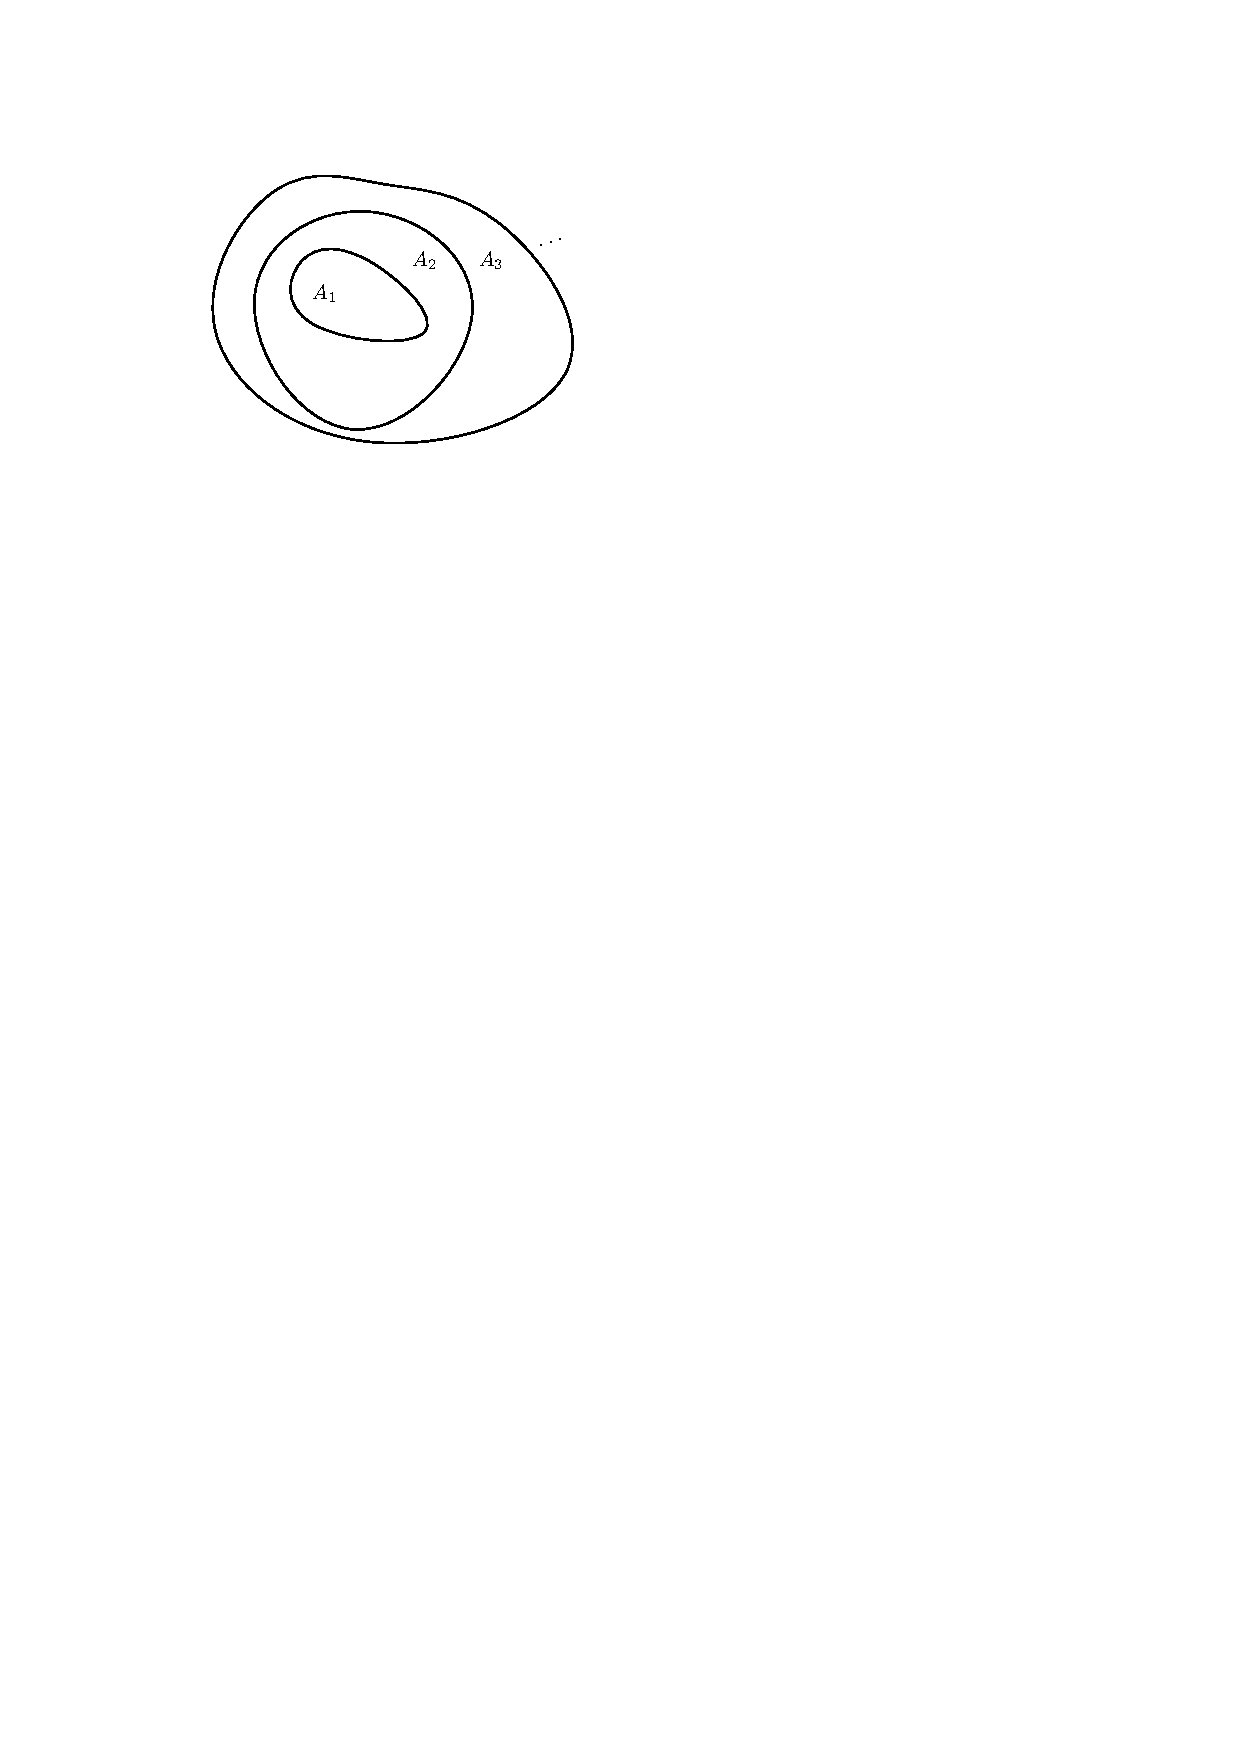
\includegraphics{ch02-neklesajici-posl-mnozin.pdf}
            \caption{Neklesající posloupnost množin}
            \label{fig:nekl-posl-mnozin}
        \end{subfigure}
        \qquad
        \begin{subfigure}{0.45\textwidth}
            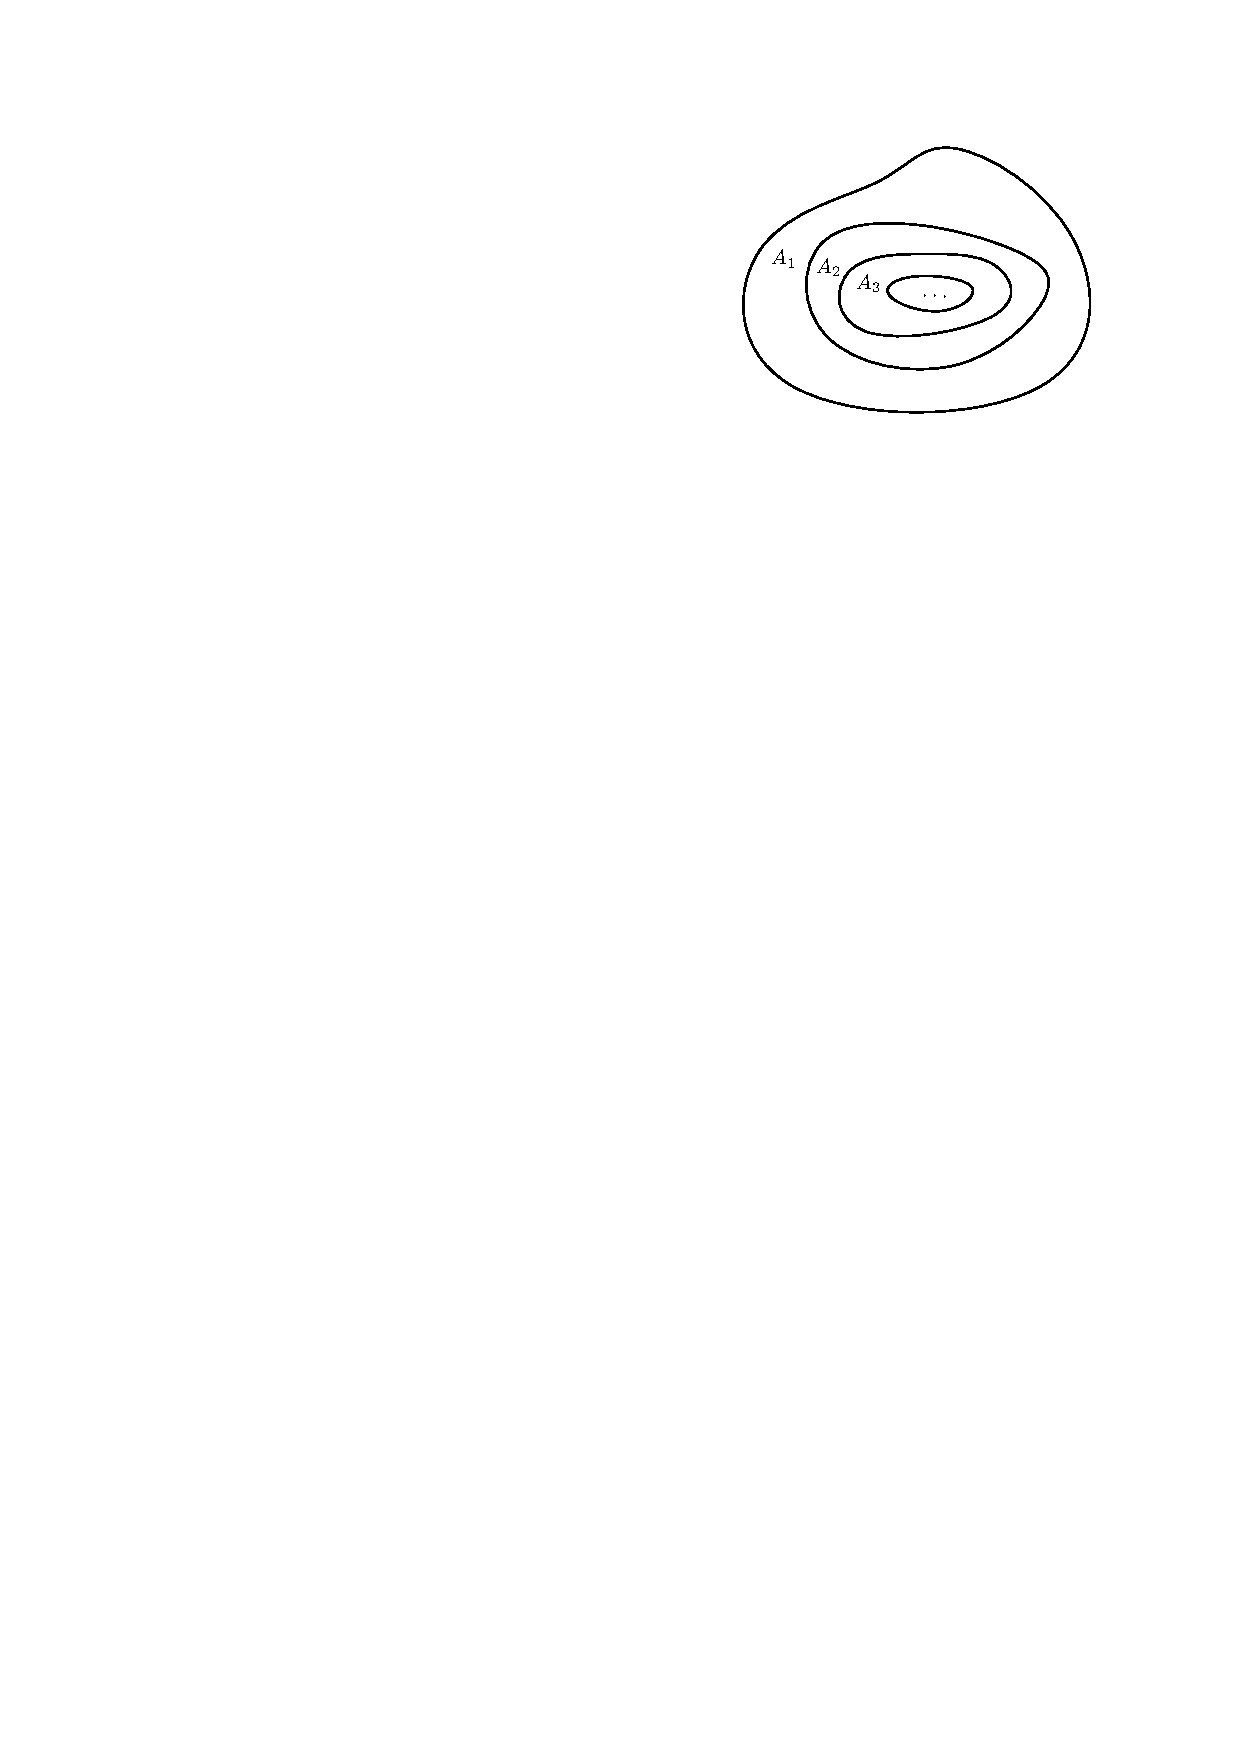
\includegraphics{ch02-nerostouci-posl-mnozin.pdf}
            \caption{Nerostoucí posloupnost množin}
            \label{fig:nerost-posl-mnozin}
        \end{subfigure}
        %% Problém s~PDF/A
        \begin{subfigure}{0.45\textwidth}
            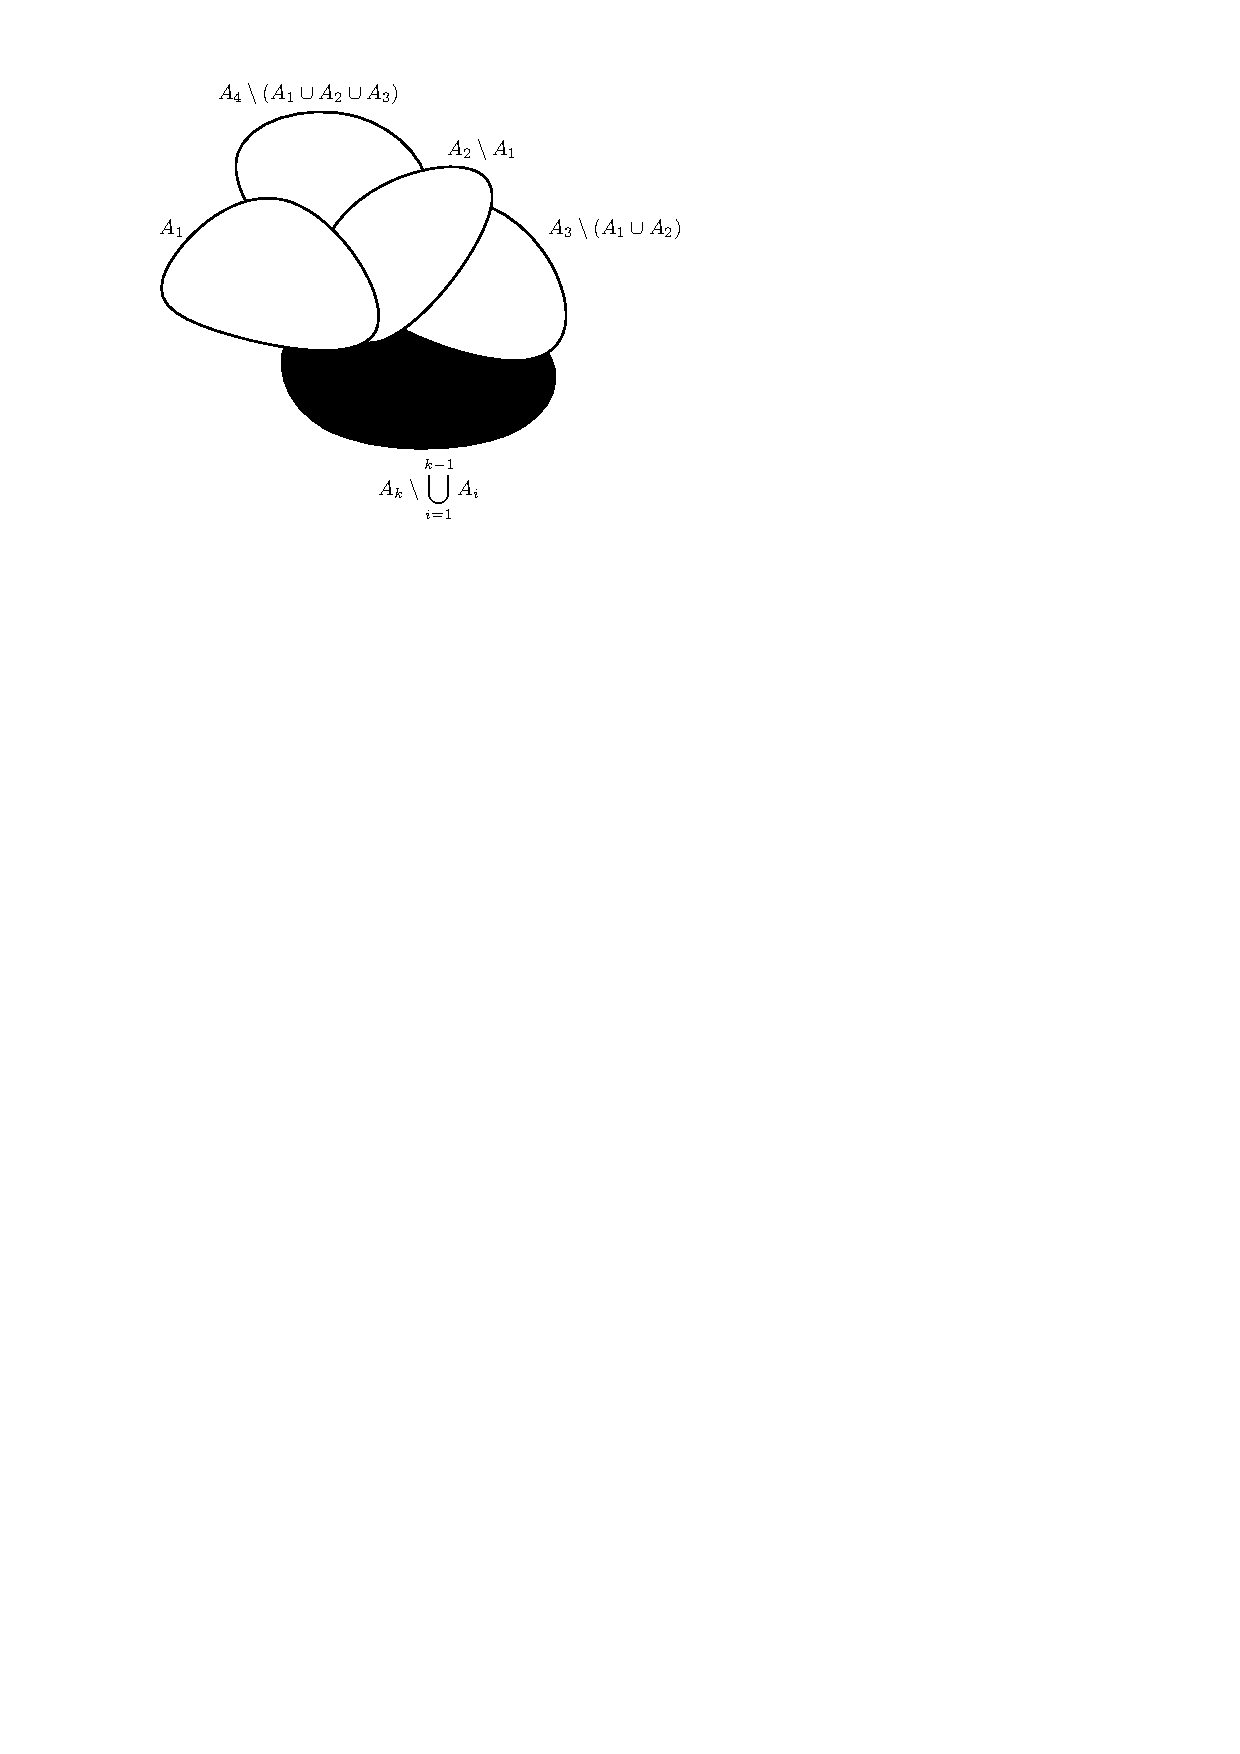
\includegraphics{ch02-vlastnosti-miry-bod-v.pdf}
            \caption{Konstrukce množin $B_k$}
            \label{fig:vlastnosti-miry-bod-v}
        \end{subfigure}
        \caption{Ilustrace k~důkazu věty \ref{thm:mira-vlastnosti}}
    \end{figure}
    (Převzato z~\citep[str. 19]{NetukaIntegral2016})
\end{proof}
\begin{remark}
    Předpoklad $\mu(A_1)<\infty$ ve větě \ref{thm:mira-vlastnosti} v~bodě \ref{thm:mira-nerost-posl} nelze vynechat. Jednoduchý protipříklad si uvedeme v~sekci \ref{sec:lebesgueova-mira}.
\end{remark}
\section{Lebesgueova míra}\label{sec:lebesgueova-mira}

\todo{Doplnit zmínku o Jordanově-Peanově obsahu}

V předešlé sekci \ref{sec:prostory-s-mirou} jsme se povídali o pojmu \emph{míra} obecně a podívali jsme se na několik příkladů. Obecnou ideu měření "velikosti" lze založit např. na aproximaci obecné množiny pomocí \emph{spočetných sjednocení útvarů}, jejichž "velikost" umíme jednoduše určit. V dalším textu se omezíme pouze na množinu $\R^n$.

Na zmíněné myšlence je postavena definice tzv. \emph{$n$-rozměrné Lebesgueovy míry}, kdy obecnou množinu budeme pokrývat pomocí \emph{kvádrů}. Připomeňme, že obecně \mbox{$n$-rozměrným} kvádrem\index{$n$-rozměrný kvádr} $I$ rozumíme kartézský součin \emph{intervalů}
\[\langle a_1,b_1\rangle,\ldots,\langle a_n,b_n\rangle\subseteq\R,\]
tj.
\[I=\prod_{i=1}^{n}\langle a_i,b_i\rangle=\langle a_1,b_1\rangle\times\langle a_2,b_2\rangle\times\dots\times\langle a_n,b_n\rangle\]
a jeho objem\index{kvádr!objem kvádru} definujeme jako
\[\vol^n(I)=\prod_{i=1}^{n}(b_i-a_i).\]
Nyní si definujeme tzv. \emph{vnější Lebesgueovu míru}.
\begin{definition}[Vnější Lebesgueova míra]\label{def:vnejsi-lebegueova-mira}
    Nechť $A\subseteq\R^n$. Pak vnější $n$-rozměr\-nou Lebesgueovou mírou\index{vnější $n$-rozměrná Lebesgueova míra} $A$ je
    \[\lambda_n^*(A)=\inf\set{\sum_{j=1}^{\infty}\vol^n(I_j)\;\middle|\;\text{$I_j$ je kvádr}\land A\subseteq\bigcup_{i=1}^\infty I_j}.\]
\end{definition}
Vnější Lebesgueova míra množiny intuitivně zachycuje informaci o "velikosti" dané množiny.  Lze ihned vidět, že pro libovolnou množinu $A\subseteq\R^n$ je $\lambda_n^*(A)\in\R_0^+$, protože $\vol^n(I_j)\geqslant0$ pro každé $j\in\N$.
\begin{example}\label{ex:lebegueova-mira-trivialni-priklady}
    Ukažme si některé triviální příklady výpočtů vnější Lebesgueovy míry z definice (viz \ref{def:vnejsi-lebegueova-mira}), tedy budeme hledat příslušné pokrytí dané množiny.
    \begin{itemize}
        \item Pro prázdnou množinu $\emptyset$ je $\lambda_n^*(\emptyset)=0$, neboť $\emptyset\subseteq\emptyset$ (tedy prázdná množina je pokrytím sebe sama) a $\vol^n(\emptyset)=0$.
        \item Mějme libovolnou konečnou množinu $A=\set{x_1,x_2,\dots,x_n}\subseteq\R^n$. Pro každé $x_j$ stačí položit $I_j=\set{x_j}$ pro každé $1\leqslant j\leqslant n$, což je degenerovaný interval, jehož objem $\vol^n(I_j)=0$.
        \item Pro libovolnou spočetnou množinu $A=\set{x_i\mid i\in\N}\subseteq\R^n$ je $\lambda_n^*(A)=0$. Pokrytí volíme stejně jako v předešlém bodě. Tedy např. pro $\Q\subset\R$ je $\lambda_1^*(\Q)=0$, neboť $\Q$ je spočetná.
        \item Pro množinu reálných čísel $\R$ je $\lambda_1^*(\R)=\infty$, avšak pro 
        \[A=\set{(x,0)\mid x\in\R}\subset\R^2\]
        (reálná osa v $\R^2$) je $\lambda_2^*(A)=0$.
    \end{itemize}
\end{example}
\begin{example}[Výpočet vnější Lebesgueovy míry intervalu]\label{ex:lebegueova-mira-delka-intervalu}
    Jako poslední si ukážeme, že vnější Lebesgueova míra v případě intervalu (ať už otevřeného, nebo uzavřeného) skutečně koresponduje s jeho délkou, tedy pro $I=(a,b)\subset\R$ je $\lambda_1^*(I)=b-a$. Zde je potřeba ukázat dvojici nerovností: $\lambda_1^*(I)\leqslant b-a$ a $\lambda_1^*(I)\geqslant b-a$.

    Zde je potřeba dávat pozor na to, že pokrytí, které hledáme, musí být spočetné. Začneme první nerovností.

    \begin{itemize}
        \item \textbf{Důkaz $\lambda_1^*(I)\geqslant b-a$.} Nechť je dána posloupnost intervalů $J_1,J_2,\ldots$, taková, že $I\subseteq\bigcup_{i=1}^\infty J_i$. Protože $(a,b)$ je otevřený interval, existuje interval $I^\prime=\langle a+\varepsilon,b-\varepsilon\rangle\subset(a,b)$ pro libovolné $\varepsilon>0$.
        
        Nechť je tedy dáno $\varepsilon>0$. Protože však interval $\langle a+\varepsilon,b-\varepsilon\rangle$ je kompaktní množina a navíc
        \[\langle a+\varepsilon,b-\varepsilon\rangle\subset(a,b)\subseteq\bigcup_{i=1}^\infty J_i\]
        lze podle Heineho-Borelovy věty (viz \todo{doplnit odkaz}) vybrat z pokrytí $J_1,J_2,\ldots$ konečné podporytí, tzn. existuje konečná posloupnost množin $J_1^\prime,J_2^\prime,\ldots,J_n^\prime$, taková, že
        \[I^\prime\subseteq\bigcup_{i=1}^\infty J_i^\prime.\]
        Z tohoto pokrytí si nyní vybereme pouze takové intervaly $J_i^\prime$, které mají neprázdný průnik s $I$, tedy
        \[J_i^\prime\cap I\neq\emptyset.\]
        Tyto intervaly si označíme $K_1,K_2,\ldots,K_m$, kde $m\leqslant n$. Není těžké si rozmyslet, že $K_1,K_2,\ldots,K_m$ tvoří opět pokrytí $I^\prime$ a navíc jejich sjednocení tvoří interval, tj.
        \[\bigcup_{i=1}^m K_i=(L,R)\supset I^\prime.\]
        Zároveň víme, že $L\leqslant a+\varepsilon$ a $R\geqslant b-\varepsilon$. Z toto tedy plyne, že
        \[\vol^1((L,R))=\sum_{i=1}^{m}\vol^1(K_i)=L-R\geqslant (b-\varepsilon)-(a+\varepsilon)=b-a-2\varepsilon.\]
        Celkově máme
        \begin{align*}
            \sum_{i=1}^{\infty}\vol^1(J_i)&\geqslant\sum_{i=1}^{n}\vol^1(J_i^\prime)\geqslant\sum_{i=1}^{m}\vol^1(K_i)\geqslant\vol^1((L,R))\\
            &=R-L\geqslant (b-\varepsilon)-(a+\varepsilon)=b-a-2\varepsilon.
        \end{align*}
        Tím je dokázána nerovnost $\lambda_1^*(I)\geqslant b-a$.
        \item \textbf{Důkaz $\lambda_1^*(I)\leqslant b-a$.} Oproti předešlému výpočtu je důkaz této části velmi snadný. Samotný interval $I=(a,b)$ tvoří totiž pokrytí sebe samotného, tzn.
        \[\lambda_1^*(I)\leqslant\vol^1((a,b))=b-a.\]
    \end{itemize}
    Z platnosti obou nerovností tedy máme, že $\lambda_1^*(I)=b-a$.
\end{example}
\begin{remark}
    Vraťme se na chvíli k větě \ref{thm:mira-vlastnosti} o vlastnostech míry, konkrétně bod \ref{thm:mira-nerost-posl}. Předpoklad $\mu(A_1)<\infty$ zde vynechat nelze. Stačí vzít množiny $A_j=\langle j,\infty)$, tzn. $\lambda_n^*(A_j)=\lambda_n^*(\langle j,\infty))=\infty$ pro každé $j\in\N$. Snadno si rozmyslíme, že
    \[\bigcap_{i=1}^\infty A_i=\emptyset,\]
    nicméně lze vidět, že zatímco $\lim_{j\to\infty}\mu(A_j)=\infty$, tak $\mu(\bigcap_{i=1}^\infty A_i)=0$.
\end{remark}

Z příkladů \ref{ex:lebegueova-mira-trivialni-priklady} a \ref{ex:lebegueova-mira-delka-intervalu} můžeme vidět, že pro rozumně zvolené množiny zachycuje vnější Lebesgueova míra jejich intuitivní "velikost". V případě intervalu odpovídá jeho délce, v případě diskrétní množiny je nulová a podobně např. pro obdélník lze ukázat, že odpovídá jeho obsahu, popř. pro kvádr jeho objemu.

Nyní se však nabízí jedna otázka. Čtenář by mohl již od chvíle, kdy jsme zavedli pojem vnější Lebesgueovy míry (opět viz definice \ref{def:vnejsi-lebegueova-mira}) namítat, co nás opravňuje nazývat zobrazení $\lambda_n^*$ mírou, tj. ve smyslu definice \ref{def:prostor-s-mirou}. Jak víme, že splňuje podmínku $\sigma$-aditivity? Na tuto otázku odpověď není zcela přímočará a vlastně není ani jednoduchá.

Bohužel pro libovolně zvolenou množinu $X$ a $\sigma$-algebru $\mathcal{A}$ v případě vnější Lebesgueovy míry obecně neplatí vlastnost aditivity, tedy existují množiny $A,B\in\mathcal{A}$, takové, že
\[\lambda_n^*(A\cup B)\neq\lambda_n^*(A)+\lambda_n^*(B).\]
Příklad takových množin využívá např. takzvaná \emph{Vitaliho konstrukce}\index{Vitaliho konstrukce}, se kterou přišel italský matematik \name{Giuseppe Vitali} (1875--1932) roku 1905, využívající invariance vnější Lebesgueovy míry vůči posunutí, tzn. $\lambda_n^*(x+A)=\lambda_n^*(A)$. \cite{OConnor2025} V rámci tohoto textu se jí zde zabývat nebudeme, avšak pro zájemce doporučuji zdroje \citep[str. 3]{Lukes2013} a \cite{Verner2025}, kde je tato konstrukce podrobněji rozepsána.

Je tedy potřeba se omezit na takové množiny, kde je $\lambda_n^*$ aditivní. Existuje více způsobů, jak lze charakterizovat takové množiny, avšak my si zde uvedeme způsob, se kterým přišel řecký matematik \name{Constantin Carathéodory} (1873--1950).
\begin{definition}[Lebesgueovská měřitelnost]\label{def:lebesgueovska-meritelnost}
    Množinu $A\subseteq\R^n$ nazveme (lebesgueovsky) měřitelnou\index{lebesgueovsky měřitelná množina}, pokud pro každou množinu $G$ platí
    \[\lambda_n^*(G)=\lambda_n^*(A\cap G)+\lambda_n^*(A\setminus G).\]
    Systém všech měřitelných množin v $R^n$ značíme $\mathcal{L}^n$.  Pokud $A\in\mathcal{L}^n$, pak číslo $\lambda_n(A)=\lambda_n^*$ nazýváme $n$-rozměrnou Lebesgueovou mírou\index{$n$-rozměrná Lebesgueova míra} množiny $A$.
\end{definition}

\todo{Musí být $G$ omezená (viz porovnání knih \emph{Real Analysis} a \emph{Measure and integral})?}
\section{Box-counting dimenze}\label{sec:box-counting-dimenze}

Tomuto typu dimenze jsme se již v~základu věnovali v~kapitole~\ref{chapter:uvod_do_fraktalu},~specificky sekci~\ref{sec:fraktalni_dimenze},~kde jsme rozebrali jeho způsob jejího výpočtu a~ukázali jsme si jej několika příkladech. V~této části si blíže rozebereme některé další vlastnosti týkající se právě \emph{box-counting dimenze}\index{box-counting dimenze}\index{dimenze!box-counting}\footnote{V kapitole~\ref{chapter:uvod_do_fraktalu} jsme pro jednoduchost používali obecnější termín \emph{fraktální dimenze}. Ten však zahrnuje daleko širší škálu možných definic,~než jen tu,~kterou jsme si představili. Avšak dále v~tomto textu budeme používat výhradně její skutečný název,~tj. box-counting dimenze.} a~pokusíme se ji lépe zasadit do kontextu teorie míry,~které jsme se samostatně až do této chvíle věnovali.

\subsection{Definice a~výpočet}\label{subsec:definice-a-vypocet-bc-dimenze}

Jako první se podíváme na myšlenku box-counting trochu blíže a~maličko si ji zobecníme. Původně jsme nahlíželi na dimenzi jako na exponent,~s nímž roste "velikost" zkoumaného útvaru. Tato myšlenka se ukázala jako rozumná,~neboť pro "klasické" geometrické útvary vycházela tato dimenze vždy celočíselně,~nicméně už tomu tak nebylo v~případě fraktálních útvarů. Podstata byla taková,~že jsme útvar $F$ rozdělili na určitý počet stejně "velkých částí",~označme $F_1,F_2,\ldots,F_m$ v~nějakém měřítku $\varepsilon>0$. Zkusme nyní požadavek na striktně stejnou velikost (formálně vzato míru) trochu rozvolnit. Bude nám stačit,~když pro každé $i$ je
\[\diam{F_i}\leqslant\delta,\;\text{kde}\;\delta>0.\]
Zároveň nebudeme požadovat,~aby množiny $F_1,F_2,\ldots,F_m$ byly všechny striktně po dvou téměř disjunktními\footnote{Množiny $M,N$ jsou \emph{téměř disjunktní},~pokud $\interior{M}\cap\interior{N}=\emptyset$,~tedy může nastat,~že se na hranici mohou "dotýkat",~tzn. $\boundary{M}\cap\boundary{N}\neq\emptyset$.} podmnožinami $F$,~ale stačí,~když budou tvořit pokrytí $F$.

Mějme tedy nějakou neprázdnoou omezenou množinu $F\subset\R^n$,~kde pro každé $\delta>0$ budeme hledat \emph{nejmenší počet} množin,~takových,~že pokrývají $F$. Toto číslo si označíme $N_\delta(F)$. Dimenze množiny $F$ by tedy měla odrážet "rychlost" růstu $N_\delta(F)$ pro $\delta\to 0^+$. Je-li splněna aproximace
\begin{equation}\label{eq:odhad-n-delta}
    N_\delta(F)\approx c\delta^{-s}
\end{equation}
pro $c>0$,~pak řekneme,~že množina $F$ má box-counting dimenzi $s$. (Převzato z~\citep[str. 27]{Falconer2014}.)
\begin{remark}
    V~dalším textu budeme místo $\delta\to 0^+$ psát pro jednoduchost pouze $\delta\to 0$,~byť by se slušilo používat první variantu. Čtenáři je však nejspíše jasné,~že uvažovat záporný průměr množiny nemá smysl.
\end{remark}
Logaritmováním a~úpravou výrazu \eqref{eq:odhad-n-delta} dostaneme:
\begin{align}\label{eq:odvozeni-box-counting-dimenze}
    \ln{N_\delta(F)}&\approx\ln{c}+\ln{\delta^{-s}}\\
    \ln{N_\delta(F)}&\approx\ln{c}-s\ln{\delta}\\
    s&\approx\dfrac{\ln{N_\delta(F)}}{-\ln{\delta}}+\dfrac{\ln{c}}{\ln{\delta}}.
\end{align}
Když porovnáme výsledek v~\eqref{eq:odvozeni-box-counting-dimenze} s~rovností \eqref{eq:fraktalni-dimenze} z~minulé kapitoly,~můžeme si všimnout,~že zde navíc figuruje člen $\ln{c}/\ln{\delta}$. Když však uvážíme limitu daného výrazu pro $\delta\to 0$,~dostaneme původní vzorec,~který jsme již viděli,~tj.
\[\lim_{\delta\to 0}\left(\dfrac{\ln{N_\delta(F)}}{-\ln{\delta}}+\dfrac{\ln{c}}{\ln{\delta}}\right)=\lim_{\delta\to 0}\dfrac{\ln{N_\delta(F)}}{-\ln{\delta}}+\lim_{\delta\to 0}\dfrac{\ln{c}}{\ln{\delta}}=\lim_{\delta\to 0}\dfrac{\ln{N_\delta(F)}}{-\ln{\delta}}.\]
% \begin{definition}[$\delta$-pokrytí]\label{def:delta-pokryti}
%     Nechť $(X,\varrho)$ je metrický prostor,~$F\subseteq X$ a~$\delta>0$. Jestliže $\mathcal{F}=\set{F_1,F_2,\ldots}\subseteq\powset{X}$ je pokrytí $F$ a~zároveň $\diam{F_j}\leqslant\delta$ pro každé $j$,~pak $\mathcal{F}$ nazýváme $\delta$-pokrytí\index{$\delta$-pokrytí} množiny $F$.
% \end{definition}
Předchozí úvahu můžeme shrnout do následující definice.
\begin{definition}[Box-counting dimenze]\label{def:box-counting-dimenze}
    Nechť $F\subset \R^n$ je neprázdná omezená množina. Pak definujeme následující:
    \begin{enumerate}[label=(\alph*)]
        \item \emph{Nejmenší počet množin v~$\delta$-pokrytí množiny $F$} značíme $N_\delta(F)$,~tj.
        \[N_\delta(F)=\min\set{m\in\N_0\;\middle|\;F\subseteq\bigcup_{i=1}^n F_i\;,\;\diam{F_j}\leqslant\delta\;\text{pro}\;1\leqslant j\leqslant m}.\]
        \item \emph{Horní box-counting dimenze}\index{box-counting dimenze!horní}\index{horní box-counting dimenze} množiny $F$ je
        \[\upperdimB{F}=\limsup_{\delta\to 0}\dfrac{\ln{N_\delta(F)}}{-\ln{\delta}}.\]
        \item \emph{Dolní box-counting dimenze}\index{box-counting dimenze!dolní}\index{dolní box-counting dimenze} množiny $F$ je
        \[\lowerdimB{F}=\liminf_{\delta\to 0}\dfrac{\ln{N_\delta(F)}}{-\ln{\delta}}.\]
    \end{enumerate}
    V~případě,~že $\lowerdimB{F}=\upperdimB{F}$,~pak společnou hodnotu nazýváme \emph{box-counting dimenzí}\index{dimenze!box-counting}\index{box-counting dimenze} množiny $F$,~značíme $\dimB{F}$,~přičemž platí
    \[\dimB{F}=\lim_{\delta\to 0}\dfrac{\ln{N_\delta(F)}}{-\ln{\delta}}.\]
\end{definition}
\begin{remark}
    Zde je důležité zmínit,~že pro v~dalším textu budeme uvažovat $\delta$ dostatečně malé,~konkrétně $0<\delta<1$,~tzn.~hodnota $-\ln{\delta}$ je~vždy kladná. Dále též budeme pracovat (podle definice~\ref{def:box-counting-dimenze}) pouze s~neprázdnými omezenými množinami,~abychom se vyhnuli problémům s~případy,~kdy $N_\delta(F)=\infty$ nebo $N_\delta(F)=0$.
\end{remark}
Abychom uvedli vše na pravou míru,~box-counting dimenzi lze taktéž definovat více způsoby. V~tuto uvažujeme obecně $\delta$-pokrytí dané množiny $F$,~tj. pokrytí \emph{obecnými} množinami o~průměru maximálně $\delta>0$. Lze se však zaměřit i~na konkrétní útvary,~jak ukazuje následující věta.
\begin{theorem}[Ekvivalentní definice box-counting dimenze]\label{thm:ekvivalentni-def-box-counting-dimenze}
    Nechť $F\subset \R^n$ je neprázdná omezená množina. Pak
    \begin{align*}
        \lowerdimB{F}&=\liminf_{\delta\to 0}\dfrac{\ln{M_\delta(F)}}{-\ln{\delta}},\\
        \upperdimB{F}&=\limsup_{\delta\to 0}\dfrac{\ln{M_\delta(F)}}{-\ln{\delta}},\\
        \dimB{F}&=\lim_{\delta\to 0}\dfrac{\ln{M_\delta(F)}}{-\ln{\delta}},
    \end{align*}
    kde $M_\delta(F)$ je definováno jedním z~následujících vzorců:
    \begin{enumerate}[label=(\roman*)]
        \item\label{thm:pokryti-delta-uz-koulemi} $\displaystyle M_\delta(F)=\inf\set{m\;\middle|\;F\subseteq\bigcup\limits_{i=1}^m K_\delta(x_i)\;,\;x_j\in\R^n\;\text{pro}\;1\leqslant j\leqslant m}$,
        \item\label{thm:pokryti-delta-kvadry} $\displaystyle M_\delta(F)=\inf\set{m\;\middle|\;F\subseteq\bigcup\limits_{i=1}^m I_i\;,\;I_j=\prod_{k=1}^{n}\langle a_k,a_k+\delta\rangle\;\text{pro}\;1\leqslant j\leqslant m}$,
        \item\label{thm:pokryti-delta-sit} $\displaystyle M_\delta(F)=\left|\set{I\;\middle|\;I\cap F\neq\emptyset\;,\;I\in\mathcal{Q}_\delta}\right|$,~kde $\delta>0$.
        \item\label{thm:pokryti-delta-dis-ot-koulemi} $\displaystyle M_\delta(F)=\sup\set{m\;\middle|\;B_\delta(x_i)\cap B_\delta(x_j)=\emptyset\;;\;x_i,x_j\in\R^n\;\text{pro}\;1\leqslant i,j\leqslant m}$.
    \end{enumerate}
\end{theorem}

Pojďme si větu~\ref{thm:ekvivalentni-def-box-counting-dimenze} nyní trochu rozebrat.
\begin{itemize}
    \item Body~\ref{thm:pokryti-delta-uz-koulemi} a~\ref{thm:pokryti-delta-dis-ot-koulemi} říkají,~že $M_\delta(F)$ je rovno \emph{nejmenšímu počtu uzavřených koulí o~poloměru $\delta$,~které pokrývají $F$},~resp. \emph{nejvyšší počet disjunktních otevřených koulí,~které mají střed v~$F$}.
    \item Podobně body~\ref{thm:pokryti-delta-kvadry} a~\ref{thm:pokryti-delta-sit} tvrdí,~že $M_\delta(F)$ lze definovat jako pokrytí kvádry o~stranách délky $\delta$,~resp. počet všech kvádrů z~$\delta$-mříže,~které mají s~$F$ neprázdný průnik.
\end{itemize}
Pro představu viz obrázek~\ref{fig:ilustrace-definic-bc-dimenze}. Důkaz věty je delší a~opět jej vynecháme,~nicméně lze jej nalézt v~knize \citep[str. 30]{Falconer2014}.
\begin{figure}
    \centering
    \begin{subfigure}{0.4\textwidth}
        \centering
        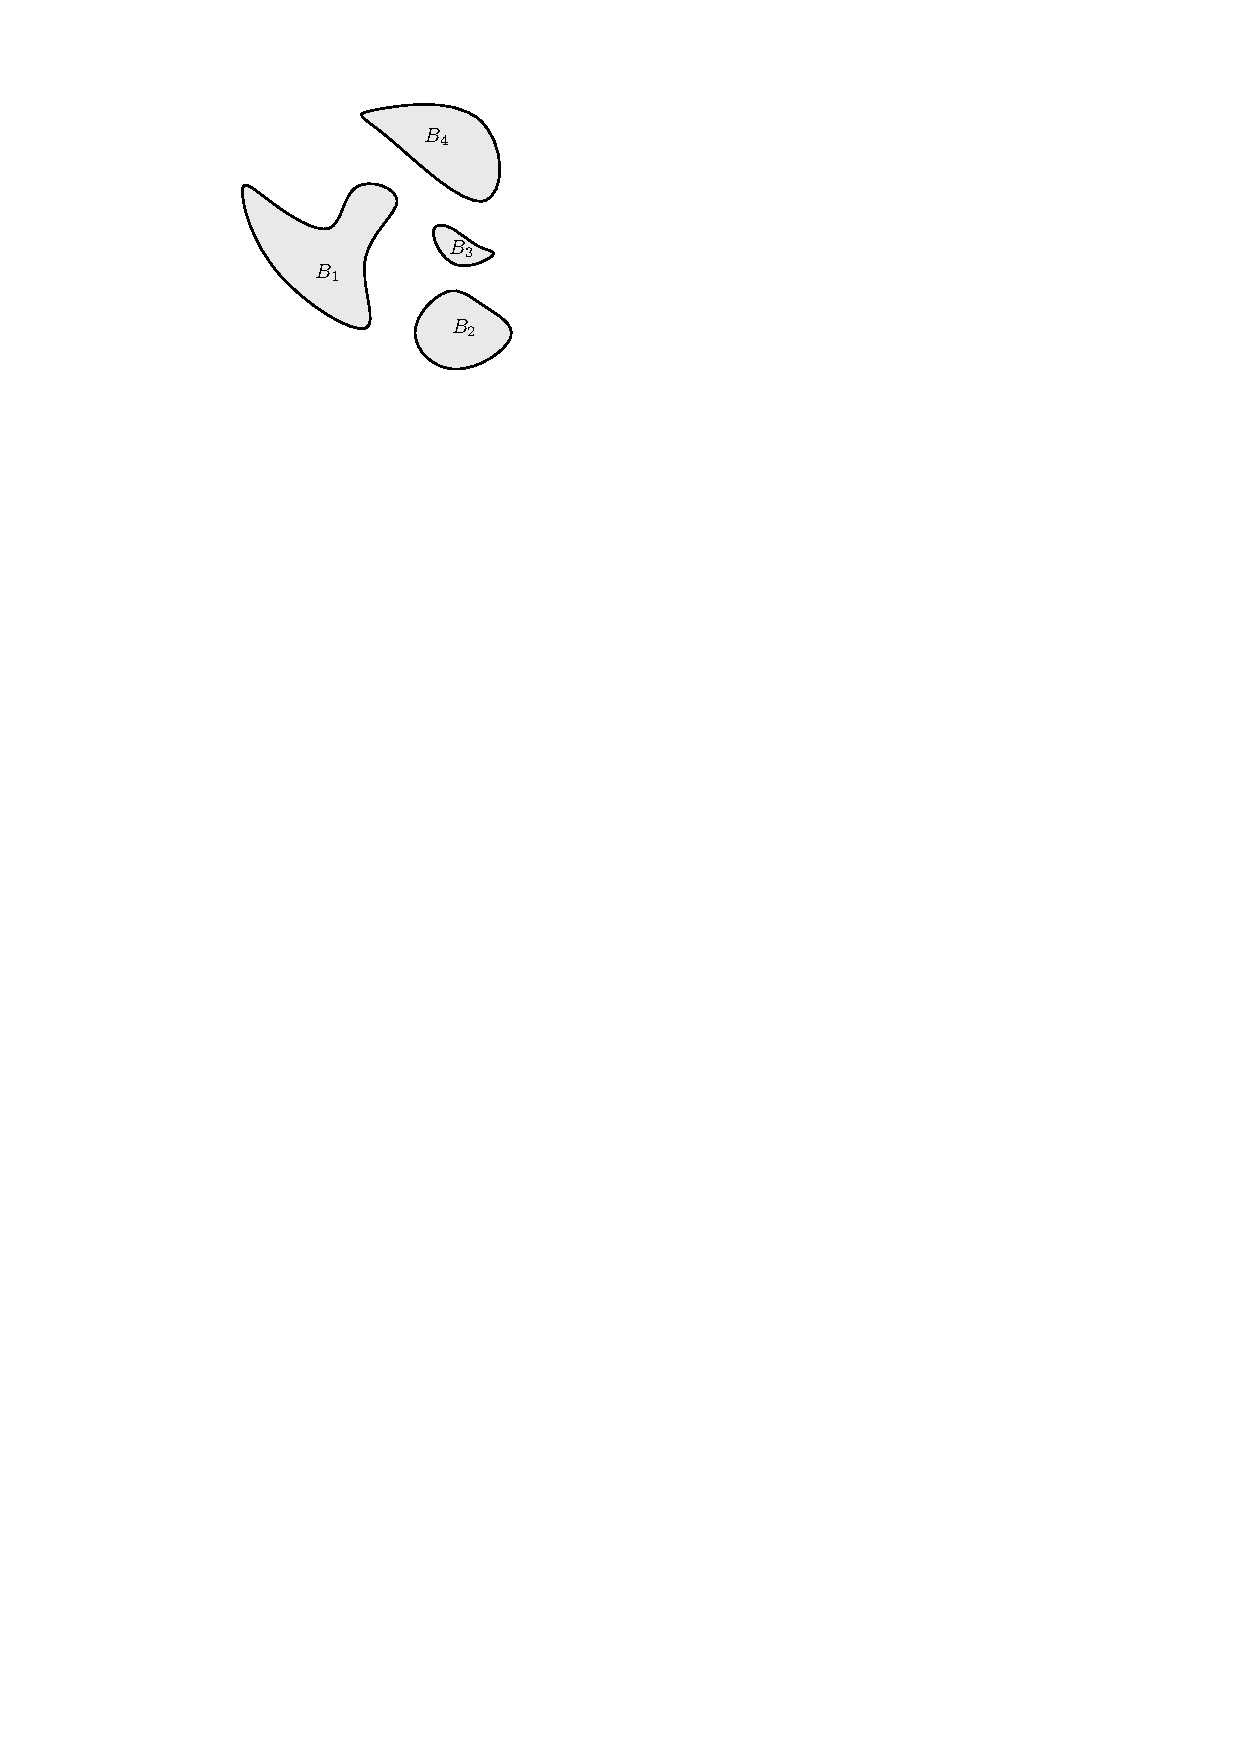
\includegraphics{ch02-bc-dimenze.pdf}
        \caption{Množina $B=\bigcup_{i=1}^4 B_i$}
        \label{subfig:bc-dimenze-pokryvana-mnozina}
    \end{subfigure}
    \qquad
    \begin{subfigure}{0.4\textwidth}
        \centering
        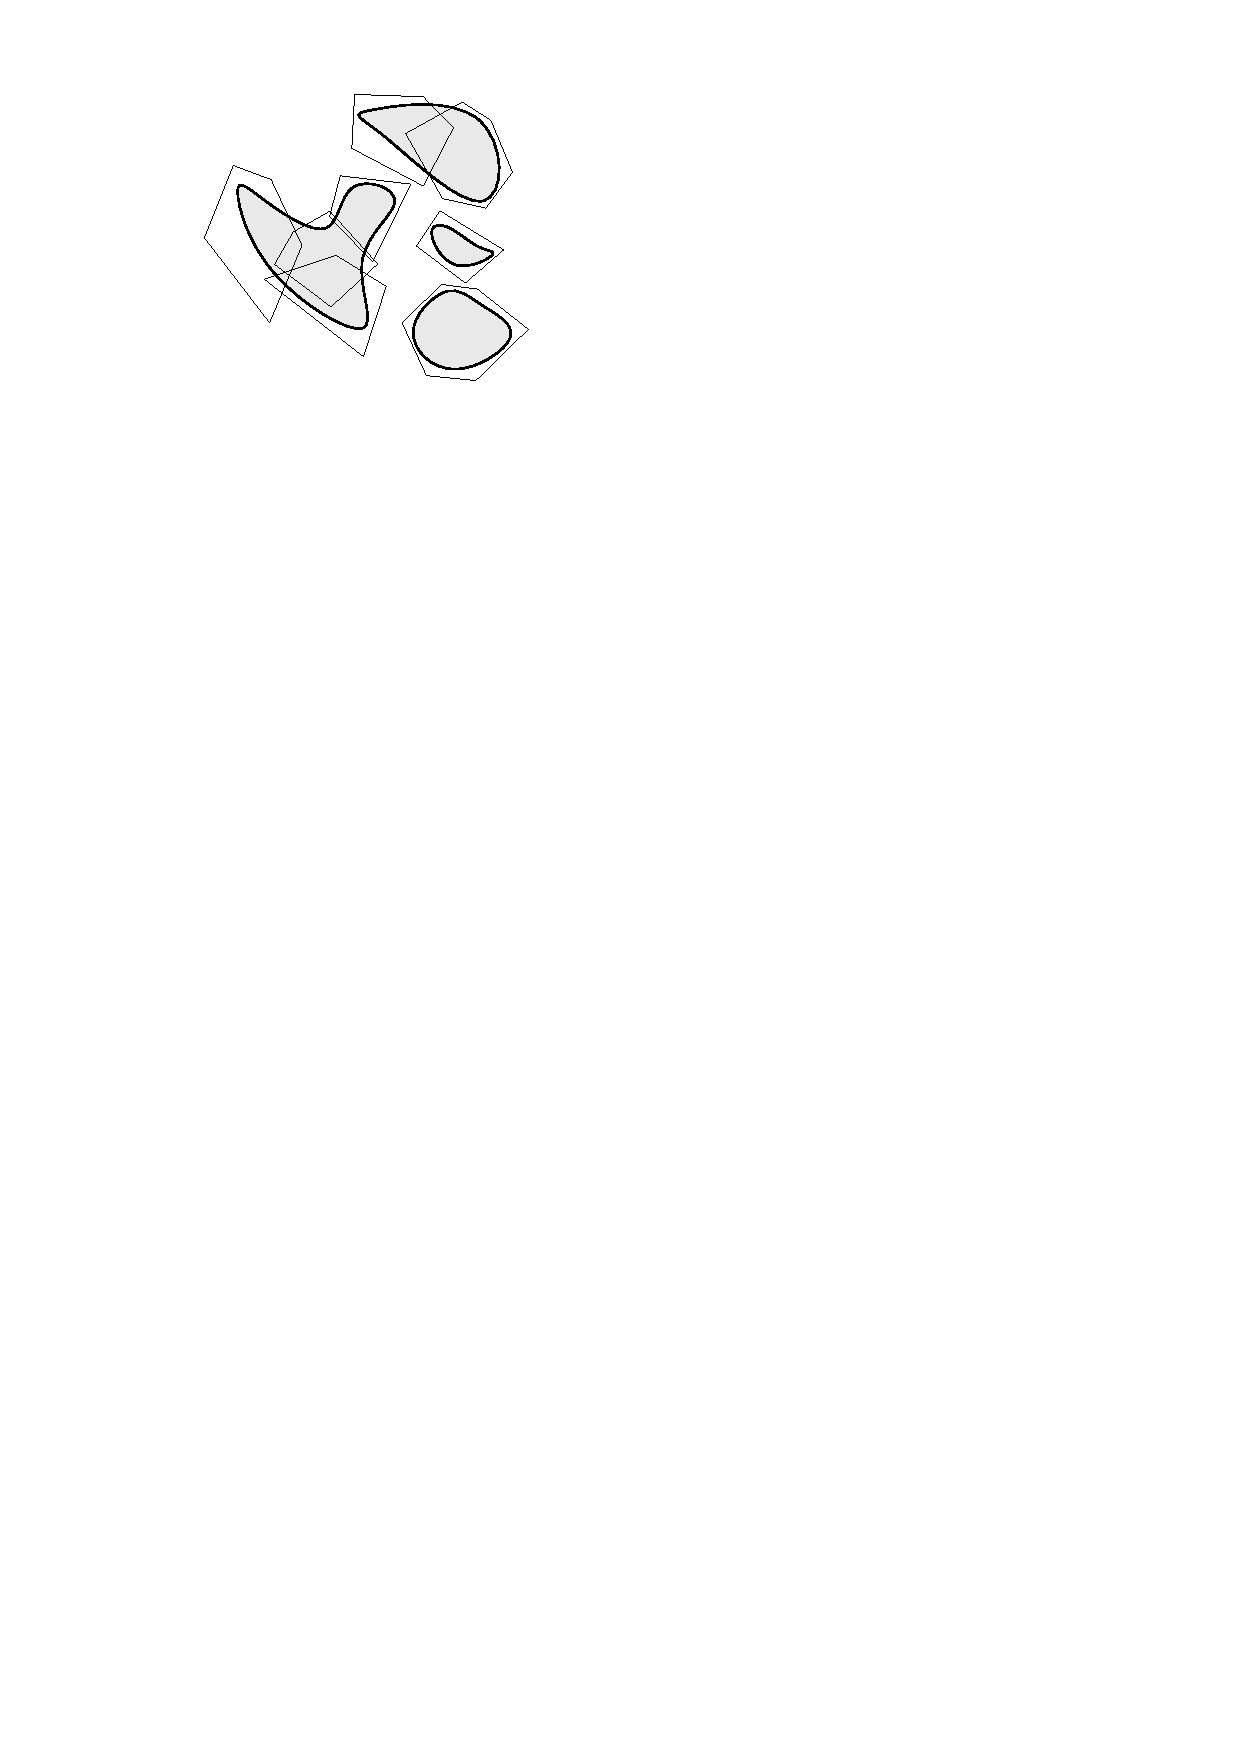
\includegraphics{ch02-bc-dimenze-delta-pokryti.pdf}
        \caption{$\delta$-pokrytí množiny $B$ (viz definice~\ref{def:box-counting-dimenze})}
        \label{subfig:bc-dimenze-delta-pokryti}
    \end{subfigure}
    \qquad
    \begin{subfigure}{0.4\textwidth}
        \centering
        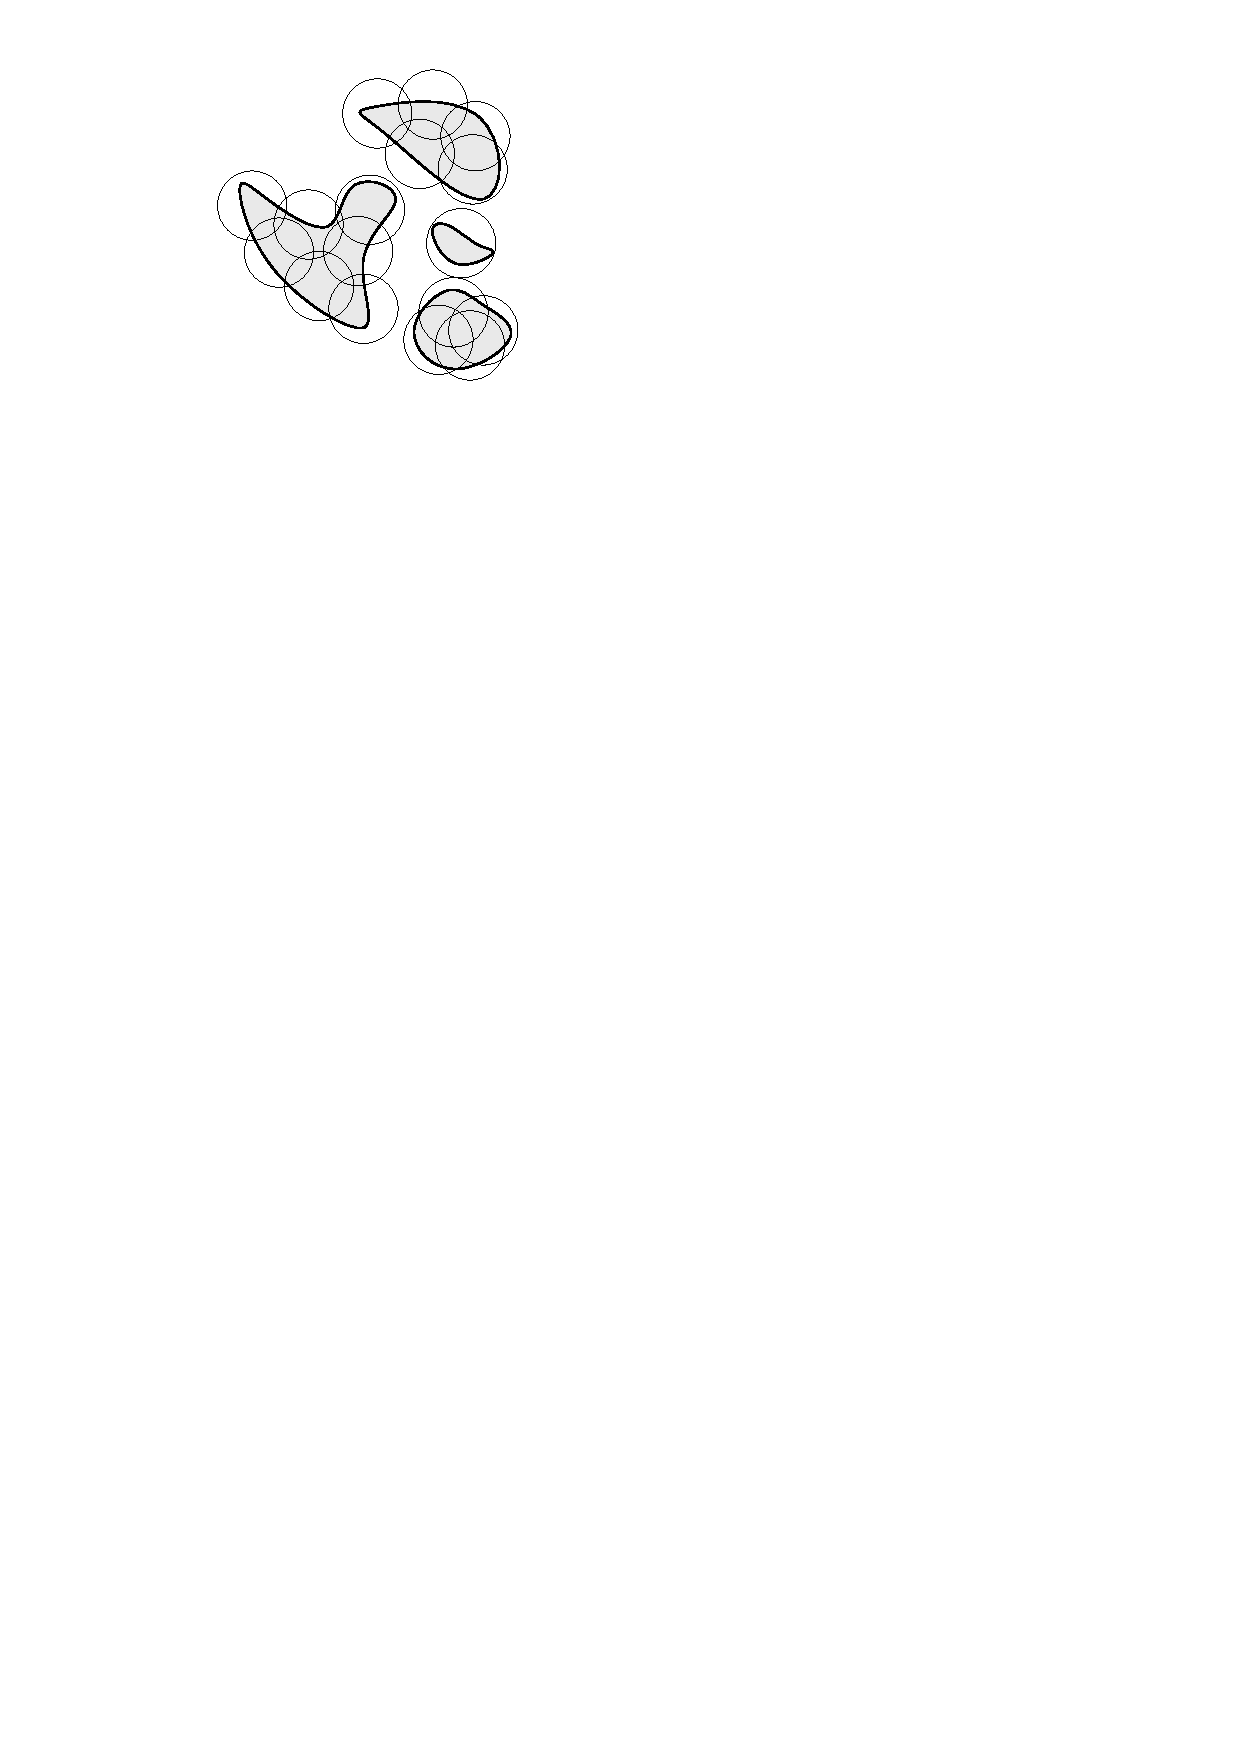
\includegraphics{ch02-bc-dimenze-pokryti-uz-koule.pdf}
        \caption{Pokrytí uzavřenými koulemi (viz bod~\ref{thm:pokryti-delta-uz-koulemi})}
        \label{subfig:bc-dimenze-uz-koule}
    \end{subfigure}
    \qquad
    \begin{subfigure}{0.4\textwidth}
        \centering
        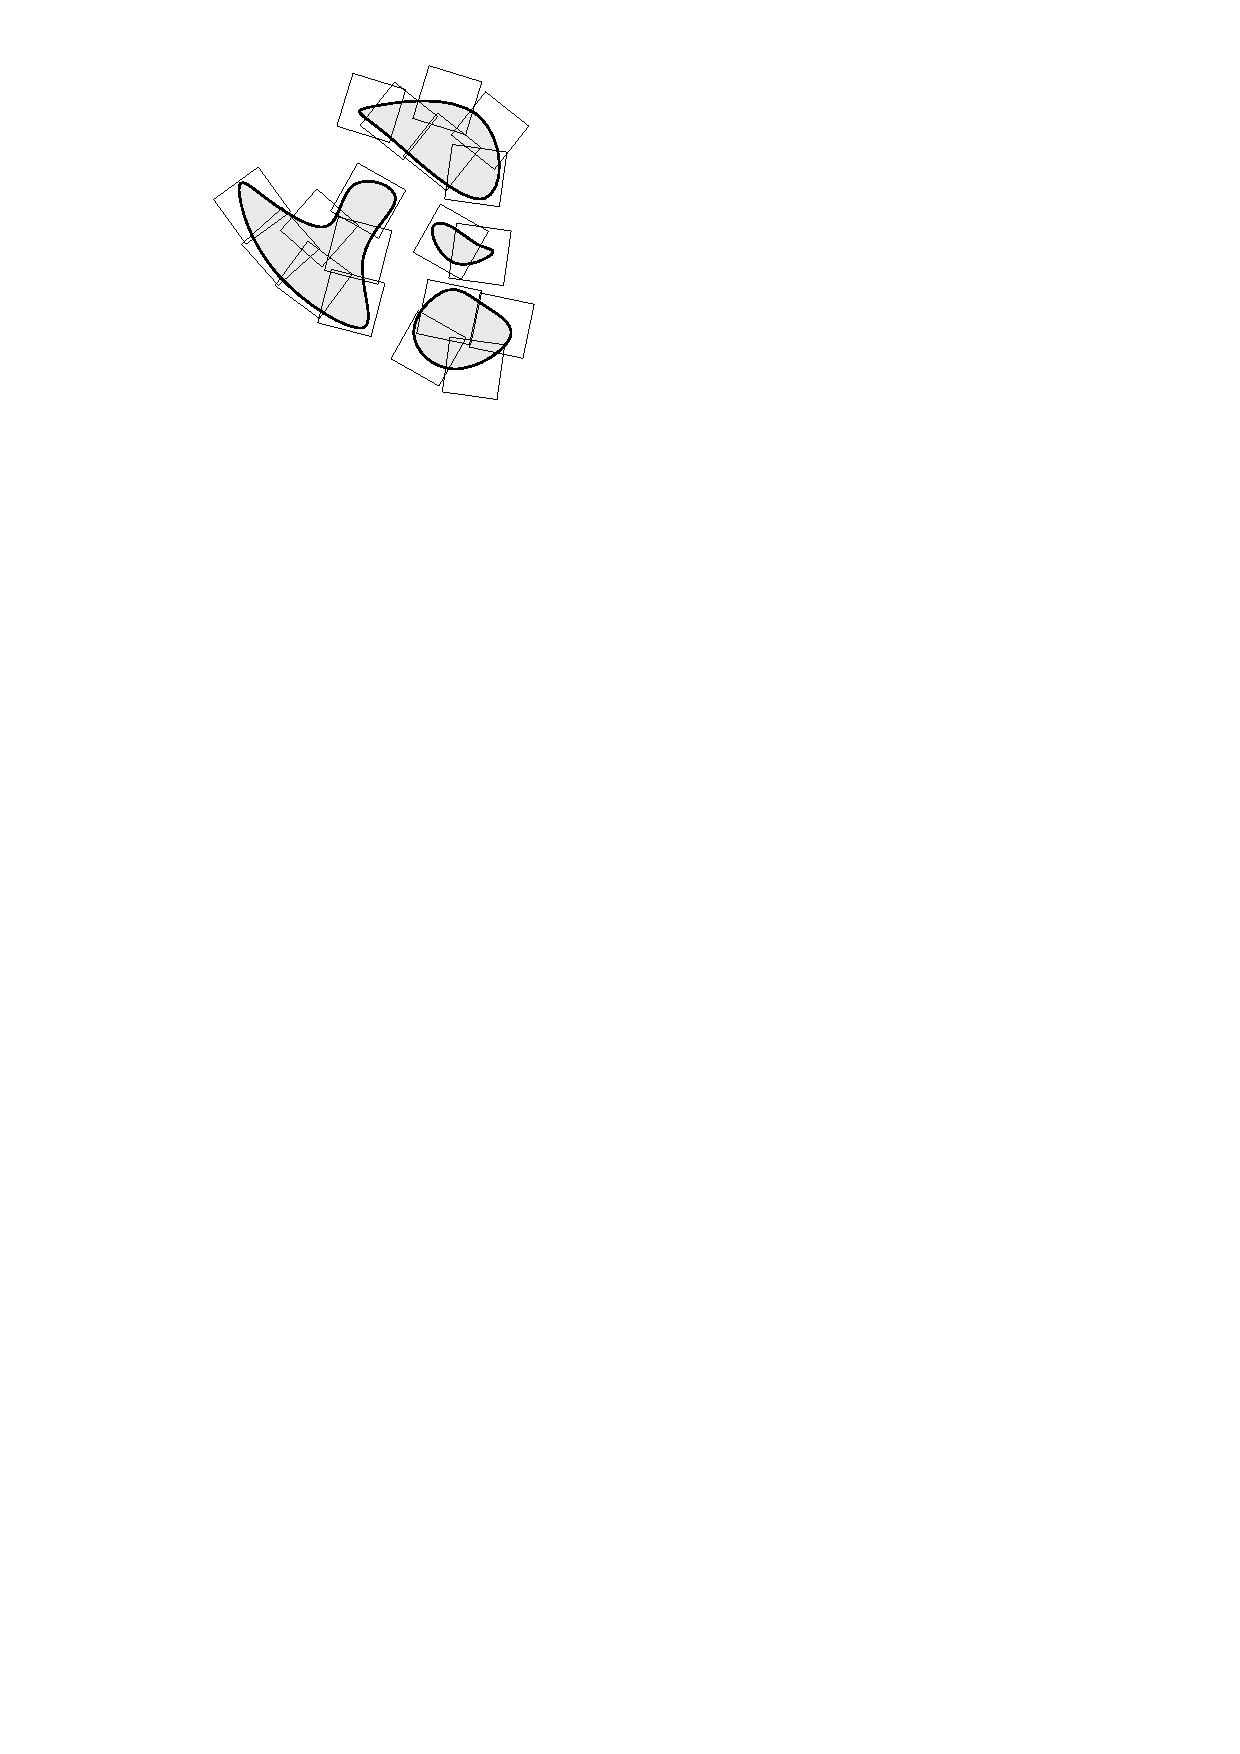
\includegraphics{ch02-bc-dimenze-pokryti-kvadry.pdf}
        \caption{Pokrytí pomocí kvádrů (viz bod~\ref{thm:pokryti-delta-kvadry})}
        \label{subfig:bc-dimenze-kvadry}
    \end{subfigure}
    \qquad
    \begin{subfigure}{0.4\textwidth}
        \centering
        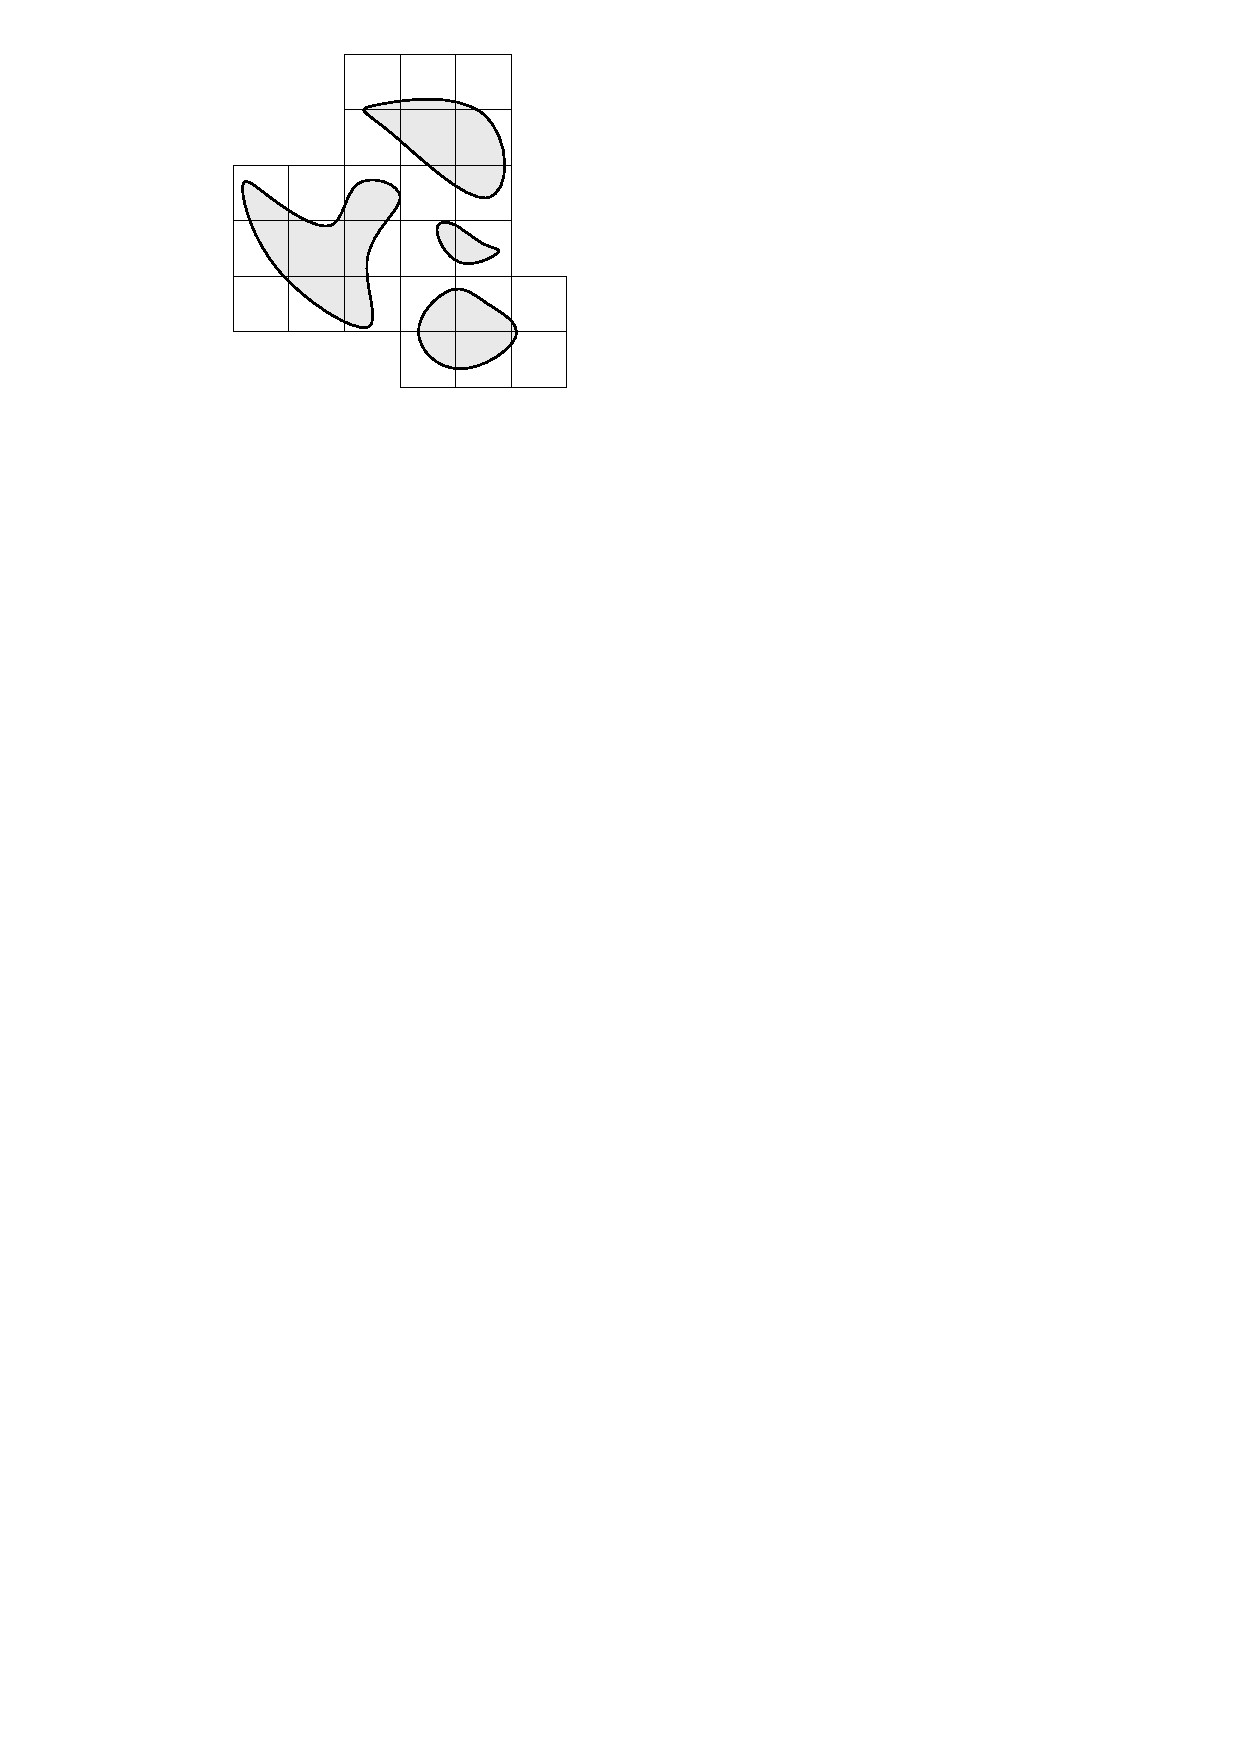
\includegraphics{ch02-bc-dimenze-pokryti-delta-sit.pdf}
        \caption{$\delta$-mříž (viz bod~\ref{thm:pokryti-delta-sit})}
        \label{subfig:bc-dimenze-delta-sit}
    \end{subfigure}
    \qquad
    \begin{subfigure}{0.4\textwidth}
        \centering
        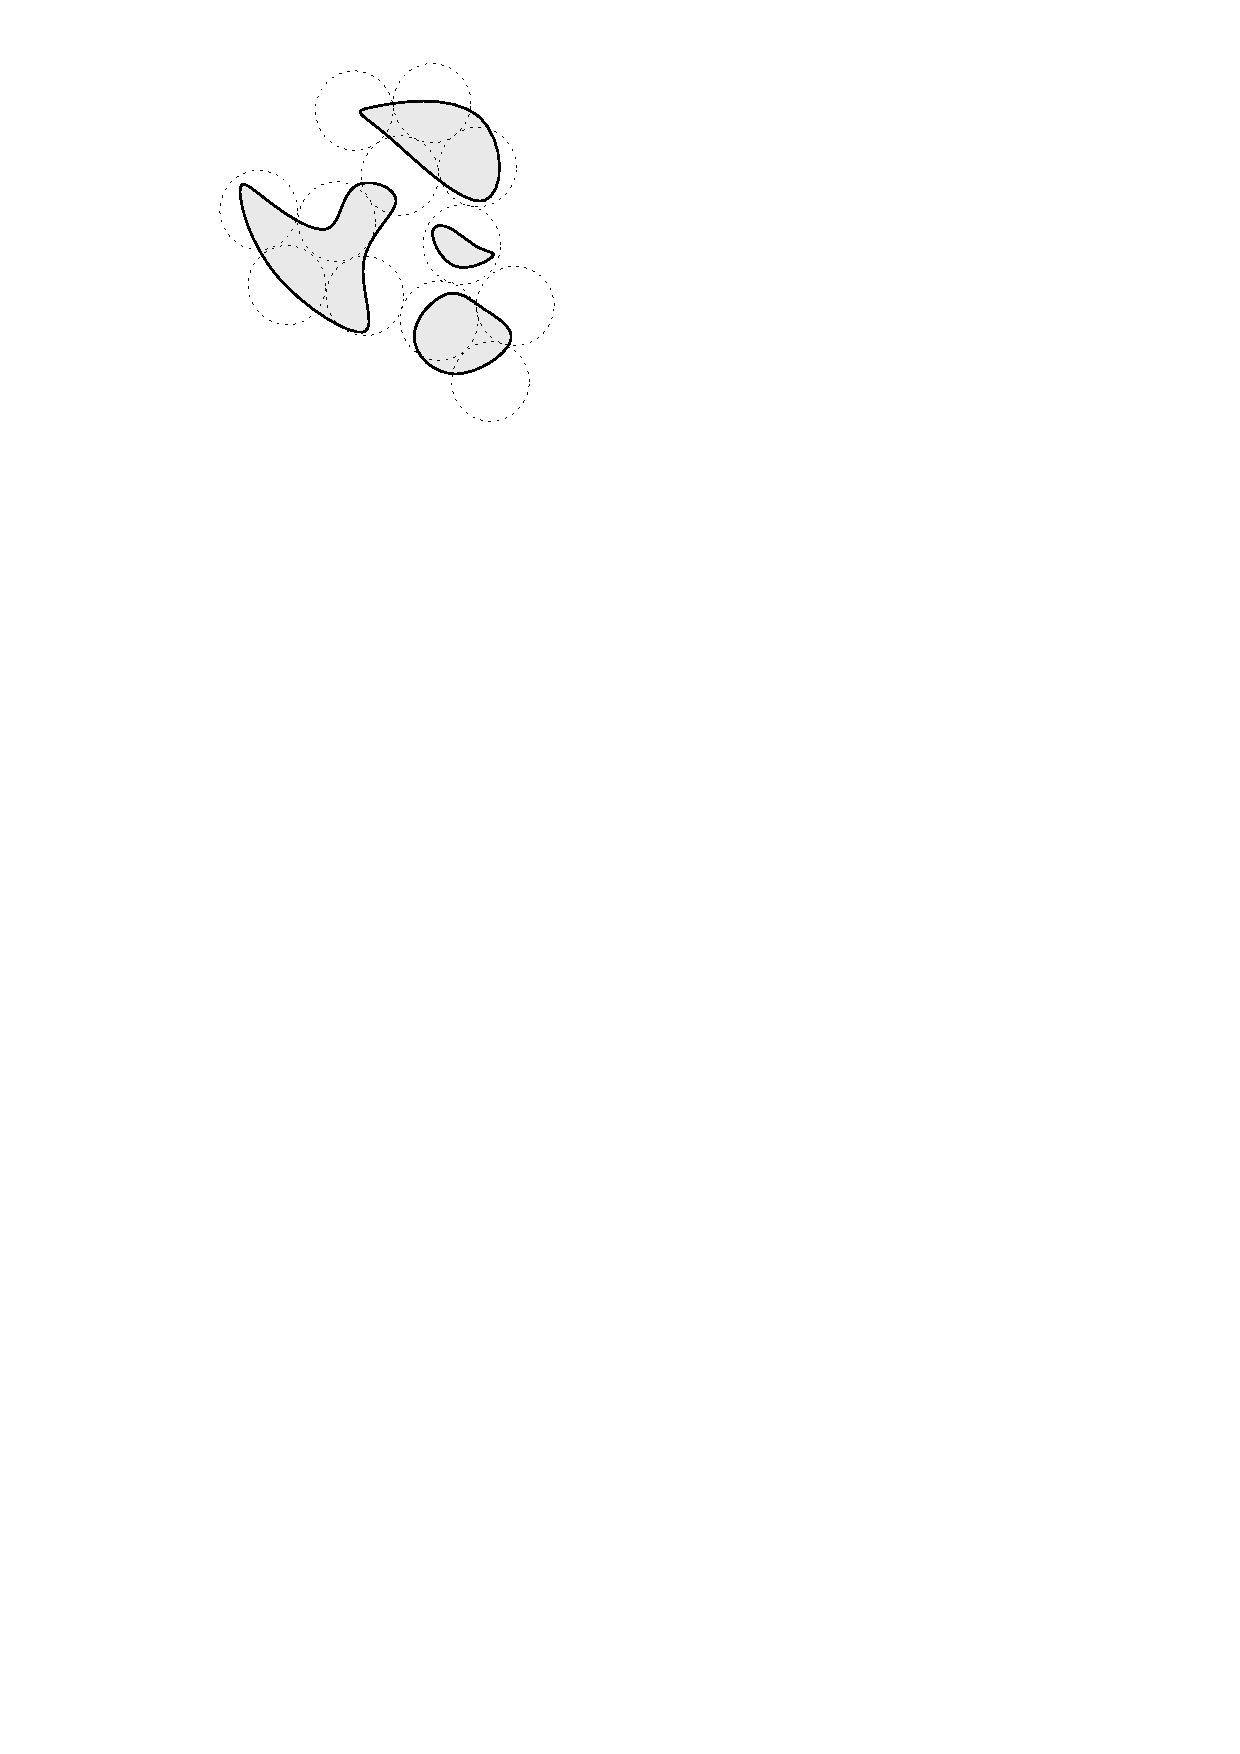
\includegraphics{ch02-bc-dimenze-pokryti-ot-koule.pdf}
        \caption{Pokrytí otevřenými po dvou disjunktními koulemi (viz bod~\ref{thm:pokryti-delta-dis-ot-koulemi})}
        \label{subfig:bc-dimenze-ot-koule}
    \end{subfigure}
    \caption[Ilustrace věty~\ref{thm:ekvivalentni-def-box-counting-dimenze}]{Ilustrace věty~\ref{thm:ekvivalentni-def-box-counting-dimenze} (Inspirováno \citep[str. 29]{Falconer2014})}
    \label{fig:ilustrace-definic-bc-dimenze}
\end{figure}

Zároveň body~\ref{thm:pokryti-delta-kvadry} a~\ref{thm:pokryti-delta-sit} nám dávají dobré opodstatnění názvu tohoto typu dimenze,~neboť v~podstatě zkoumáme pokrývání daného obrazce "kostkami". Při aproximacích box-counting dimenze obrazce $F\subset\R^2$ tak lze pracovat s~mřížkou čtverců o~libovolné straně $\delta>0$,~kdy $M_\delta(F)$ stanovíme jako počet čtverců,~které se překrývají se zkoumaným obrazcem $F$. Když se tedy zpět vrátíme k~otázce rozebírané v~úvodu tohoto textu týkající se délky pobřeží (viz kapitola~\ref{chapter:uvod_do_fraktalu}),~lze jeho "fráktálnost" do jisté míry vyjádřit právě popsaným způsobem (viz obrázek~\ref{fig:aproximace-delky-pobrezi-vb}).
\begin{figure}
    \centering
    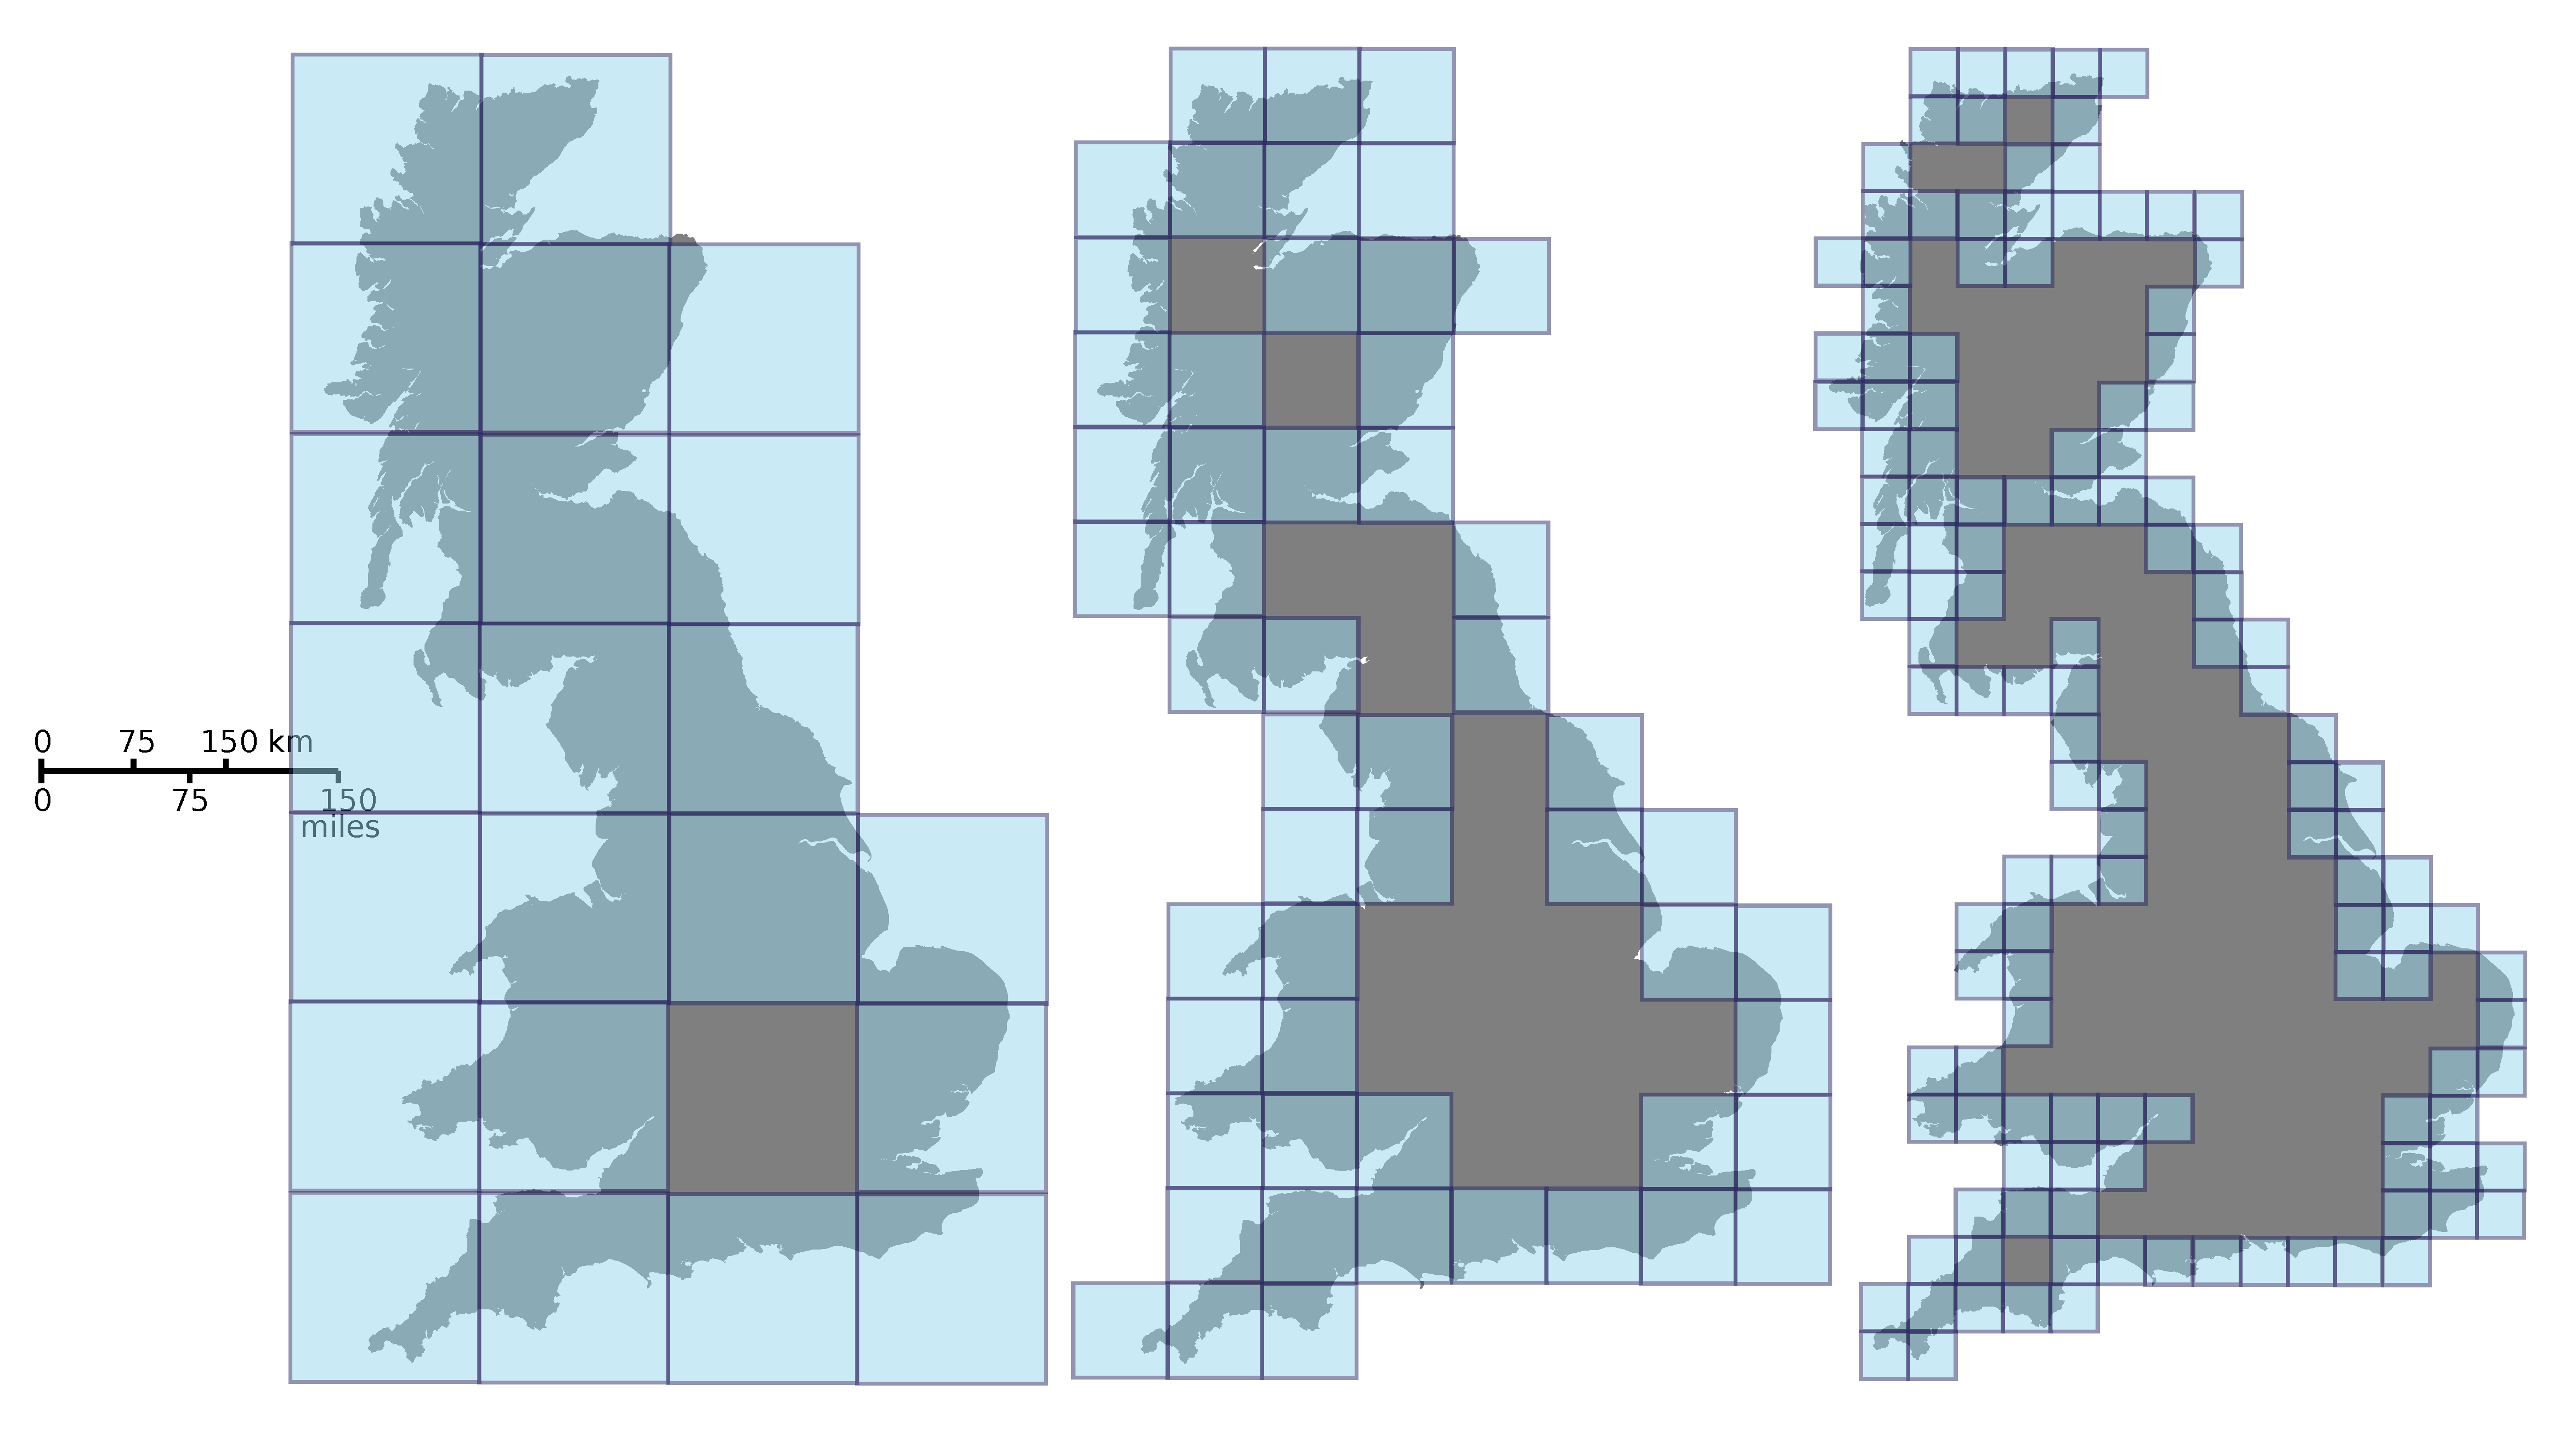
\includegraphics[width=\textwidth]{Great_Britain_Box.pdf}
    \caption[Aproximace box-counting dimenze pobřeží Velké Británie]{Aproximace box-counting dimenze pobřeží Velké Británie (Převzato z~Wikipedia Commons)\footnotemark}
    \label{fig:aproximace-delky-pobrezi-vb}
\end{figure}
Nyní se opět vrátíme k~fraktálům\footnotetext{Viz též \url{https://en.wikipedia.org/wiki/Minkowski\%E2\%80\%93Bouligand\_dimension}.} a~výpočtům jejich dimenze,~čemuž jsme se věnovali již v~sekci~\ref{sec:fraktalni_dimenze} kapitoly~\ref{chapter:uvod_do_fraktalu},~konkrétně~\ref{subsec:dimenze-fraktalu}. Tentokrát však budeme postupovat přímo podle definice box-counting dimenze~\ref{def:box-counting-dimenze},~tedy budeme zvlášť zkoumat horní a~dolní box-counting dimenzi.
\begin{example}[Cantorovo diskontinuum]\label{ex:cantorovo-diskontinuum}
    Formálně můžeme popsat Cantorovo diskontinuum $C$ jako průnik množin $C_k$ pro $k=0,1,2,\ldots$,~přičemž
    \[C_k=\bigcup _{j=0}^{3^{k-1}-1}\left(\left\langle{\frac {3j+0}{3^{k}}},{\frac {3j+1}{3^{k}}}\right\rangle\cup \left\langle{\frac {3j+2}{3^{k}}},{\frac {3j+3}{3^{k}}}\right\rangle\right).\]
    $C_k$ tedy reprezentuje $k$-tou iteraci a~$C=\bigcap_{k=0}^\infty C_k$. Již jsme měli možnost se přesvědčit,~že tento fraktál má box-counting dimenzi $\ln{2}/\ln{3}$. Zkusme nyní výpočet zopakovat,~avšak vzlášť vypočítáme $\lowerdimB{C}$ a~$\upperdimB{C}$ podíváme se,~zda se shodují.

    Jako první provedeme horní odhad. Je potřeba zvolit $\delta$ a~na jeho základě dopočítat $N_\delta(C)$. V~$k$-té iteraci,~kde $k=0,1,2,\ldots$,~bude obecně $2^k$ intervalů,~každý o~délce $(1/3)^k$,~tedy pokud zvolíme $3^{-k}<\delta\leqslant 3^{-k+1}$,~pak intervaly o~délce nejvýše $\delta$ (viz věta~\ref{thm:ekvivalentni-def-box-counting-dimenze},~bod~\ref{thm:pokryti-delta-uz-koulemi}) tvoří $\delta$ pokrytí,~přičemž $N_\delta(C)\leqslant 2^k$. Tedy celkově pro $\delta$-pokrytí všech intervalů bude potřeba nejvýše $N_\delta(C)\leqslant 2^k$ intervalů $I_1,I_2,\ldots,I_{N_\delta(C)}$ o~průměru $3^{-k}<\diam{F_i}\leqslant 3^{-k+1}$ pro každé $i$. Z~toho dostáváme
    \[\upperdimB{C}=\limsup_{\delta\to 0}\dfrac{\ln{N_\delta(C)}}{-\ln{\delta}}\leqslant\limsup_{k\to\infty}\dfrac{\ln{2^k}}{-\ln{3^{-k+1}}}=\limsup_{k\to\infty}\dfrac{k\ln{2}}{(k-1)\ln{3}}=\dfrac{\ln{2}}{\ln{3}}.\]
    Naopak pokud uvážíme intervaly délky $3^{-k-1}\leqslant\delta<3^{-k}$,~pak každý z~nich má neprázdný průnik s~maximálně jedním intervalem $k$-té iterace $C$. Těch je,~jak již víme,~$2^k$,~tedy intervalů $I_1,I_2,\ldots,I_{N_\delta(C)}$ bude nejméně $2^k$ pro pokrytí $C$,~tzn. $N_\delta(C)\geqslant 2^k$. Tím dostáváme dolní odhad:
    \[\lowerdimB{C}=\liminf_{\delta\to 0}\dfrac{\ln{N_\delta(C)}}{-\ln{\delta}}\geqslant\liminf_{\delta\to 0}\dfrac{\ln{2^k}}{-\ln{3^{-k-1}}}=\liminf_{\delta\to 0}\dfrac{k\ln{2}}{(k+1)\ln{3}}=\dfrac{\ln{2}}{\ln{3}}.\]

    Protože $\lowerdimB{C}=\upperdimB{C}=\ln{2}/\ln{3}$,~tak box-counting dimenze Cantorova diskontinua je $\dimB{C}=\ln{2}/\ln{3}$. (Převzato z~\citep[str. 32]{Falconer2014})
\end{example}
Podobně bychom postupovali pro rovinné obrazce.
\begin{example}[Kochova křivka]\label{ex:kochova-krivka}
    Zde se zatím s~formální definicí nebudeme zatěžovat. Opět ukážene horní a~dolní odhad zvlášť. Kochovu křivku si označíme $K$.

    Obecně $k$-tá iterace Kochovy křivky bude obsahovat $4^n$ úseček,~každá o~délce $(1/3)^k$. Podobně jako v~předchozím příkladu~\ref{ex:cantorovo-diskontinuum} zvolíme $3^{-k}<\delta\leqslant 3^{-k+1}$. Pokud si pro pokrytí zvolíme uzavřené koule
    \[K_\delta^1(x_1),K_\delta^2(x_2),\ldots,K_\delta^{M_\delta(K)}(x_{M_\delta(K)}),\;\text{kde}\;x_1,x_2,\ldots,x_{M_\delta(K)}\in\R^2\]
    pak $M_\delta(K)\leqslant 4^k$. Tedy
    \[\upperdimB{K}=\limsup_{\delta\to 0}\dfrac{\ln{M_\delta(K)}}{-\ln{K}}\leqslant\limsup_{k\to\infty}\dfrac{\ln{4^k}}{-\ln{3^{-k+1}}}=\limsup_{k\to\infty}\dfrac{k\ln{4}}{(k-1)\ln{3}}=\dfrac{\ln{4}}{\ln{3}}.\]

    Podobně pro dolní odhad uvážíme $3^{-k-1}\leqslant\delta<3^{-k}$. Vezmeme-li uzavřené koule $K_\delta^1(x_1),K_\delta^2(x_2),\ldots,K_\delta^{M_\delta(K)}(x_{M_\delta(K)})$,~pak žádný nemůže mít neprázdný průnik s~více než čtyřmi úsečkami,~tedy pro jejich pokrytí je zapotřebí alespoň $M_\delta(K)\geqslant 4^k/4=4^{k-1}$,~čímž dostáváme
    \[\lowerdimB{K}=\liminf_{\delta\to 0}\dfrac{\ln{M_\delta(K)}}{-\ln{K}}\geqslant\liminf_{k\to\infty}\dfrac{\ln{4^{k-1}}}{-\ln{3^{-k-1}}}=\liminf_{k\to\infty}\dfrac{(k-1)\ln{4}}{(k+1)\ln{3}}=\dfrac{\ln{4}}{\ln{3}}.\]
    Tzn.~$\dimB{K}=\ln{4}/\ln{3}$.
\end{example}
\begin{remark}
    Obecně množina $F$ skládající se z~$m$ disjunktních kopií sebe samotné,~kde každá z~nich je $r$-krát menší,~má dimenzi $\dimB{F}=\ln{m}/\ln{r}$.
\end{remark}
Nyní se podíváme ještě na jedno možné pojetí box-counting dimenze. Připomeňme,~že $\delta$-okolím množiny $F$ v~metrickém prostoru $(X,\varrho)$ rozumíme
\[(F)_\delta=\set{x\in X\mid\exists y\in X: \varrho(x,y)<\delta}.\]
Budeme nyní sledovat,~jak "rychle" se mění objem $(F)_\delta$ pro $\delta\to 0$. A~se zmínkou objemu nám zde do hry opět vstupuje Lebesgueova míra $\lebesguemeasure{n}$,~o níž jsme si povídali v~sekci~\ref{sec:lebesgueova-mira}. Podívejme se nejdříve na několik příkladů.
\begin{itemize}
    \item Pro konečnou množinu $F=\set{x_1,x_2,\ldots,x_n}$ je
    \[\lebesguemeasure{3}((F)_\delta)\leqslant n\cdot\dfrac{4}{3}\pi\delta^3.\]
    Pro $\delta\leqslant1/2\min\set{\varrho(x,y)\mid x,y\in F}$ nastává rovnost.
    \item Pro úsečku $u\subset\R^3$ o~délce $\ell$ lze objem jejího $\delta$-okolí stanovit jako
    \[\lebesguemeasure{3}((u)_\delta)=\dfrac{4}{3}\pi \delta^3+\pi\delta^2\ell.\]
    Pokud však uvážíme $\delta$ dostatečně malé,~lze první člen zanedbat a~psát
    \[\lebesguemeasure{3}((u)_\delta)\approx\pi\ell\delta^2.\]
    \item V~případě neprázdného kvádru
    \[I=\set{(x,y,0)\mid x\in\langle a_1,b_1\rangle\,,\,y\in\langle a_2,b_2\rangle}\]
    je
    \begin{align*}
        \lebesguemeasure{3}(I_\delta)&=2(b_1-a_1)(a_2-b_2)\delta+2(b_1-a_1)\pi\delta^2+2(b_2-a_2)\pi\delta^2+\dfrac{4}{3}\pi\delta^3\\
        &\approx 2(b_1-a_1)(a_2-b_2)\delta
    \end{align*}
    \item Pro kouli $B_r(x)\subset\R^3$,~kde $x\in\R^3$ a~$r>0$ je objem
    \[\lebesguemeasure{3}((B_r(x))_\delta)=\dfrac{4}{3}\pi (r+\delta)^3=\dfrac{4}{3}\pi r^3+4\pi r^2\delta+4\pi r\delta^2+\dfrac{4}{3}\pi\delta^3\approx\dfrac{4}{3}\pi r^3.\]
    Změna objemu je v~tomto případě vzhledem k~původnímu objemu zanedbatelná.
\end{itemize}
Výsledky si srovnejme v~tabulce~\ref{table:odhady-lambda_3}.
\begin{table}[h]
    \centering
    \begin{tabular}{r|D{=}{=}{-1}}
    Útvar $F$                               & \multicolumn{1}{c}{$\lebesguemeasure{3}((F)_\delta)$}       \\\hline
    Konečná množina $\set{x_1,\ldots,x_n}$     & \frac{4n}{3}\pi\delta^3=c_1\delta^3   \\
    Úsečka $u$                             & \pi\ell\delta^2=c_2\delta^2           \\
    Kvádr $I$                              & 2(b_1-a_1)(a_2-b_2)\delta=c_3\delta^1 \\
    Koule $B_\delta(x)$                    & \frac{4}{3}\pi r^3=c_4\delta^0      
    \end{tabular}
    \caption{Odhady $\lebesguemeasure{3}$ pro vybrané útvary}
    \label{table:odhady-lambda_3}
\end{table}
Můžeme si všimnout,~že v~každém případě odhad objemu vychází $\lebesguemeasure{3}((F)_\delta)\approx c\delta^{3-s}$,~kde $c>0$ je závislé na původní míře $F$ a~$s$ udává dimenzi. Obecněji pro množinu $F\subseteq\R^n$ bychom došli k~$\lebesguemeasure{n}((F)_\delta)\approx c\delta^{n-s}$. Nyní,~podobně jako v~úvodu této sekce,~zkusme opět vyjádřit $s$:
\begin{align*}
    \ln{\lebesguemeasure{n}((F)_\delta)}&\approx\ln{c}+(n-s)\ln{\delta}\\
    s\ln{\delta}&\approx n\ln{\delta}-\ln{\lebesguemeasure{n}((F)_\delta)}+\ln{c}\\
    s&\approx n-\dfrac{\ln{\lebesguemeasure{n}((F)_\delta)}}{\ln{\delta}}+\dfrac{\ln{c}}{\ln{\delta}}.
\end{align*}
Poslední člen bude v~limitě opět nulový.

Lze ukázat,~že $s$ není v~tomto případě nic jiného,~než již námi zkoumaná\linebreak{}box-counting dimenze. To si shrneme a~dokážeme ve větě~\ref{thm:bc-dimenze-lebesgueova-mira}.
\begin{theorem}\label{thm:bc-dimenze-lebesgueova-mira}
    Nechť $F\subseteq\R^n$. Pak platí: 
    \begin{enumerate}[label=(\roman*)]
        \item $\lowerdimB{F}=n-\limsup\limits_{\delta\to 0}\dfrac{\ln{\lebesguemeasure{n}((F)_\delta)}}{\ln{\delta}}$,
        \item $\upperdimB{F}=n-\liminf\limits_{\delta\to 0}\dfrac{\ln{\lebesguemeasure{n}((F)_\delta)}}{\ln{\delta}}$.
    \end{enumerate}
\end{theorem}
\begin{proof}
    V~rámci důkazu využijeme větu~\ref{thm:ekvivalentni-def-box-counting-dimenze}.

    Mějme $F\subseteq\R^n$. Označme $v_n$ objem jednotkové koule $K_1(x)$\footnote{Objem koule v~$\R^n$ lze vyjádřit vztahem
    \[V_n(r)=\dfrac{\pi^{n/2}}{\Gamma\left(\frac{n}{2}+1\right)}r^n,\]
    kde $\Gamma$ je tzv. \emph{gamma funkce}. Se vzorcem však dále v~textu pracovat nebudeme.
    } v~$\R^n$ pro $x\in\R^n$ libovolné. Dále mějmě pokrytí
    \[\mathcal{K}=\set{K_\delta^1(x_1),K_\delta^2(x_2),\ldots,K_\delta^{M_\delta(F)}(x_{M_\delta(F)})}\]
    množiny $F$,~kde $0<\delta<1$ a~$x_j\in F$ pro každé $1\leqslant j\leqslant M_\delta(F)$,~přičemž $M_\delta(F)$ je definováno podle bodu~\ref{thm:pokryti-delta-uz-koulemi} věty~\ref{thm:ekvivalentni-def-box-counting-dimenze}. Pak lze zvolit pokrytí
    \[\mathcal{K}^\prime=\set{K_{2\delta}^1(x_1),K_{2\delta}^2(x_2),\ldots,K_{2\delta}^{M_\delta(F)}(x_{M_\delta(F)})},\]
    tzn.~$\mathcal{K}$ je zjemnění pokrytí $\mathcal{K}^\prime$. Zároveň však platí,~že $\mathcal{K}^\prime$ je i~pokrytím $(F)_\delta$. Pro libovolné $x\in (F)_\delta$ existuje totiž $y\in F$,~takové,~$\varrho(x,y)<\delta$. Tedy pro dané $y$ existuje nějaká koule $K_\ell(x_\ell)\in\mathcal{K}$,~taková,~že $y\in K_\ell(x_\ell)$,~což znamená,~že
    \[\varrho(x_\ell,y)\leqslant\varrho(x_\ell,x)+\varrho(x,y)\leqslant\delta+\delta=2\delta.\]
    Tzn.~míru $F$ lze zhora odhadnout jako
    \[\lebesguemeasure{n}((F)_\delta)\leqslant M_\delta(F)v_n(2\delta)^n.\]
    Úpravou získáme:
    \begin{align*}
        \ln{\lebesguemeasure{n}((F)_\delta)}&\leqslant n\ln{\delta}+\ln{M_\delta(F)}+\ln{2^nv_n}\\
        \dfrac{\ln{\lebesguemeasure{n}((F)_\delta)}}{-\ln\delta}&\leqslant -n+\dfrac{\ln{M_\delta(F)}}{-\ln\delta}+\dfrac{\ln{2^nv_n}}{-\ln\delta},
    \end{align*}
    tedy v~limitě
    \[\liminf_{\delta\to 0}\dfrac{\ln\lebesguemeasure{n}((F)_\delta)}{-\ln\delta}\leqslant -n+\lowerdimB{F}.\]
    K~odhadu $\upperdimB{F}$ lze dospět analogicky.

    Nyní uvažujme po dvou disjunktní otevřené koule $B_\delta^j(x_j)$,~kde $x_j\in F$ pro $1\leqslant j\leqslant M_\delta(F)$. Pak součtem jejich objemů získáme
    \[M_\delta(F)v_n\delta^n\leqslant\lebesguemeasure{n}((F)_\delta).\]
    Obdobnou úpravou této nerovnosti získáme požadovanou nerovnost.
\end{proof}
Zkusme si aplikaci věty ilustrovat opět na příkladu fraktálu.
\begin{example}[Cantorovo diskontinuum potřetí]\label{ex:cantorovo-diskontinuum-potreti}
    Pro Cantorovo diskontinuum v~$k$-té iteraci,~označme $C_k$,~lze odhadnout délku $(C_k)_\delta$ pro $3^{-k-2}\leqslant\delta\leqslant 3^{-k-1}$ jako
    \[\lebesguemeasure{1}((C_k)_\delta)\geqslant 2^k(3^{-k-2}+2\delta)\leqslant2^k\cdot 3\cdot 3^{-k-2}=2^k\cdot 3^{-k-1}.\]
    Tedy podle věty~\ref{thm:bc-dimenze-lebesgueova-mira}
    \begin{align*}
        \upperdimB{C}&=n-\liminf_{\delta\to 0}\dfrac{\ln{\lebesguemeasure{1}((C)_\delta)}}{\ln{\delta}}\leqslant1-\liminf_{k\to\infty}\dfrac{\ln{2^{k}\cdot 3^{-k-1}}}{\ln{3^{-k-1}}}\\
        &=\liminf_{k\to\infty}\dfrac{k\ln{2}}{(k+1)\ln{3}}=\dfrac{\ln{2}}{\ln{3}}.
    \end{align*}

    Podobně zvolíme-li $3^{-k-1}\leqslant\delta\leqslant 3^{-k}$,~pak
    \[\lebesguemeasure{1}((C_k)_\delta)\leqslant 2^k(3^{-k}+2\delta)\leqslant2^k\cdot 3\cdot 3^{-k}=2^k\cdot 3^{-k+1}\]
    a~tedy
    \begin{align*}
        \lowerdimB{C}&=n-\limsup_{\delta\to 0}\dfrac{\ln{\lebesguemeasure{1}((C)_\delta)}}{\ln{\delta}}\geqslant 1-\limsup_{k\to\infty}\dfrac{\ln{2^{k}\cdot 3^{-k+1}}}{\ln{3^{-k+1}}}\\
        &=\limsup_{k\to\infty}\dfrac{k\ln{2}}{(k-1)\ln{3}}=\dfrac{\ln{2}}{\ln{3}}.
    \end{align*}
\end{example}

\subsection{Vlastnosti}\label{subsec:vlastnosti-bc-dimenze}

V minulé podsekci~\ref{subsec:definice-a-vypocet-bc-dimenze} jsme se bavili o~možnostech pojetí box-counting dimenze. S~tím souvisely zejména pak věty~\ref{thm:ekvivalentni-def-box-counting-dimenze} a~\ref{thm:bc-dimenze-lebesgueova-mira}. Nyní trochu blíže ještě prozkoumáme některé její vlastnosti,~na něž se podíváme ve větě~\ref{thm:vlastnosti-bc-dimenze}.
\begin{theorem}[Vlastnosti box-counting dimenze]\label{thm:vlastnosti-bc-dimenze}
    Nechť jsou dány $F,G\subseteq\R^n$.
    \begin{enumerate}[label=(\roman*)]
        \item\label{thm:monotonie-bc-dimenze} Pokud $G\subseteq F$,~pak $\lowerdimB{G}\leqslant\lowerdimB{F}$ a~$\upperdimB{G}\leqslant\upperdimB{F}$.\rightnote{monotonie}
        \item\label{thm:rozsah-hodnot-bc-dimenze} Je-li $F\neq\emptyset$ omezená,~pak $0\leqslant\lowerdimB{F}\leqslant\upperdimB{F}\leqslant n$.\rightnote{rozsah hodnot}
        \item\label{thm:stabilita-bc-dimenze} $\upperdimB(F\cup G)=\max\set{\upperdimB{F},\upperdimB{G}}$.\rightnote{stabilita}
    \end{enumerate}
\end{theorem}
\begin{proof}
    \begin{enumerate}[label=\textit{(\roman*)}]
        \item Plyne triviálně z~faktu,~že pro libovolné $\delta>0$ je $N_\delta(G)\leqslant N_\delta(F)$,~neboť každé $\delta$-pokrytí $\mathcal{F}\supset F$ je zároveň $\delta$-pokrytím $G$.
        \item První dvojice nerovností je zjevná z~definice (viz~\ref{def:box-counting-dimenze}). Pro třetí nerovnost zvolme kvádr $I$,~takový,~že $F\subset I$. Zvolíme-li $\delta>0$ a~$\delta$-mříž $\mathcal{Q}_\delta$,~pak
        \begin{align*}
            M_\delta(F)&=\left|\set{J\;\middle|\;J\cap F\neq\emptyset\;,\;J\in\mathcal{Q}_\delta}\right|\\
            &\leqslant \left|\set{J\;\middle|\;J\cap I\neq\emptyset\;,\;J\in\mathcal{Q}_\delta}\right|\\
            &=M_\delta(I)\leqslant c\delta^{-n},
        \end{align*}
        kde $c>0$. Poslední nerovnost si lze snadno rozmyslet. Tedy podle věty~\ref{thm:ekvivalentni-def-box-counting-dimenze} a~přechozího bodu~\ref{thm:monotonie-bc-dimenze} máme
        \[\upperdimB{F}\leqslant\upperdimB{I}=\limsup_{\delta\to 0}\dfrac{\ln{N_\delta(I)}}{-\ln{\delta}}\leqslant\limsup_{\delta\to 0}\dfrac{\ln{c\delta^{-n}}}{-\ln{\delta}}=n.\]
        \item Pro $\delta>0$ volme $\delta$-pokrytí $\mathcal{F}\supset F$ a~$\mathcal{G}\supset G$. Je celkem zjevné,~že $N_\delta(F\cup G)\leqslant N_\delta(F)+N_\delta(G)$,~neboli
        \begin{align*}
            \ln(N_\delta(F)+N_\delta(G))&\leqslant \ln\left(2\max\set{N_\delta(F),N_\delta(G)}\right)\\
            &=\ln{2}+\ln\left(\max\set{N_\delta(F),N_\delta(G)}\right).
        \end{align*}
        Tedy
        \begin{align*}
            \upperdimB(F\cup G)&\leqslant\limsup_{\delta\to 0}\left(\dfrac{\ln{2}}{-\ln{\delta}}+\dfrac{\ln\left(\max\set{N_\delta(F),N_\delta(G)}\right)}{-\ln{\delta}}\right)\\
            &\leqslant\limsup_{\delta\to 0}\dfrac{\ln\left(\max\set{N_\delta(F),N_\delta(G)}\right)}{-\ln{\delta}}\\
            &=\limsup_{\delta\to 0}\left(\max\set{\dfrac{\ln{N_\delta(F)}}{-\ln{\delta}},\dfrac{\ln{N_\delta(G)}}{-\ln{\delta}}}\right)\\
            &\leqslant\max\set{\limsup_{\delta\to 0}\dfrac{\ln{N_\delta(F)}}{-\ln{\delta}},\limsup_{\delta\to 0}\dfrac{\ln{N_\delta(G)}}{-\ln{\delta}}}\\
            &=\max\set{\upperdimB{F},\upperdimB{G}}.
        \end{align*}
        Opačná nerovnost plyne z~faktu,~že $F\subset F\cup G$ a~$G\subset F\cup G$,~tedy
        \[\upperdimB(F\cup G)\geqslant\upperdimB{F}\;\text{a}\;\upperdimB(F\cup G)\geqslant\upperdimB{G}\]
        podle bodu~\ref{thm:monotonie-bc-dimenze},~neboli
        \[\upperdimB(F\cup G)=\max\set{\upperdimB{F},\upperdimB{G}}.\]
    \end{enumerate}
\end{proof}
(Převzato a~upraveno z~\citep[str. 35]{Falconer2014}.)

Poslední bod~\ref{thm:stabilita-bc-dimenze} tvrzení~\ref{thm:vlastnosti-bc-dimenze} lze pochopitelně rozšířit indukcí. Čtenář se sám může přesvědčit,~že se jedná o~relativně jednoduché cvičení.
\begin{corollary}\label{cor:stabilita-bc-dimenze-obecne}
    Pro $F_1,F_2,\ldots,F_m\subseteq\R^n$ platí:
    \[\upperdimB\left(\bigcup_{i=1}^m F_i\right)=\max\set{\upperdimB{F_j}\mid 1\leqslant j\leqslant m}.\]
\end{corollary}
\begin{proof}
    Pro $m=1$ a~$m=2$ víme,~že tvrzení platí. Pro $m+1$ lze psát:
    \begin{align*}
        \upperdimB\left(\bigcup_{i=1}^{m+1}F_i\right)&=\upperdimB\left(\left(\bigcup_{i=1}^{m}F_i\right)\cup F_{m+1}\right)\\
        &=\max\set{\upperdimB\left(\bigcup_{i=1}^{m+1}F_i\right),\upperdimB{F_{m+1}}}\\
        &\stackrel{\text{I.P.}}{=}\max\set{\max\set{\upperdimB{F_i}\mid 1\leqslant i\leqslant m},\upperdimB{F_{m+1}}}\\
        &=\max\set{\upperdimB{F_j}\mid 1\leqslant j\leqslant m+1}.
    \end{align*}
\end{proof}

Jako poslední se ještě nabízí otázka,~jak se bude dimenze $\dimB$ chovat vůči zobrazením. V~tomto kontextu pro nás budou relevantní především \emph{lipschitzovská}\index{zobrazení!lipschitzovské}\index{lipschitzovské zobrazení} a~\emph{bilipschitzovská zobrazení}\index{zobrazení!bilipschitzovské}\index{bilipschitzovské zobrazení}. Připomeňme,~že lipschitzovské zobrazení je takové zobrazení $\mapping{f}{X}{Y}$ mezi metrickými prostory $(X,\varrho_1)$ a~$(Y,\varrho_2)$,~že existuje konstanta $K>0$,~taková,~že pro každé $x,y\in X$ platí
\[\varrho_2(f(x),f(y))\leqslant K\varrho_1(x,y).\]
Pokud navíc platí,~že existují konstanty $K_1,K_2>0$,~takové,~že platí
\[K_1\varrho_1(x,y)\leqslant\varrho_2(f(x),f(y))\leqslant K_2\varrho_1(x,y),\]
pak $f$ nazýváme bilipschitzovské.

Než se však podíváme na samotný vztah box-counting dimenze a~lipschitzovských,~resp. bilipschitzovských zobrazení,~dokážeme si jedno jednoduché\linebreak{}lemma,~které později využijeme.
\begin{lemma}\label{lem:lipschitzovska-zobrazeni-a-bijekce}
    Nechť $(X,\varrho_1),(Y,\varrho_2)$ jsou metrické prostory a~zobrazení $\mapping{f}{X}{Y}$ je bilipschitzovské. Pak $\mapping{f}{X}{f(X)}$ je bijekce.
\end{lemma}
\begin{proof}
    Podle předpokladu je $f$ bilipschitzovské zobrazení,~tedy existují pro konstanty $K_1,K_2>0$,~takové,~že
    \[K_1\varrho_1(x,y)\leqslant\varrho_2(f(x),f(y))\leqslant K_2\varrho_1(x,y),\;x,y\in X.\]
    Surjektivita zobrazení $f$ je zřejmá z~její definice. Pro spor předpokládejme,~že $f$ není injektivní,~tedy existují $x,y\in X$,~taková,~že $x\neq y$ a~$f(x)=f(y)$. Pak
    \[0<K_1\varrho_1(x,y)\leqslant\varrho_2(f(x),f(y))=0,\]
    což je spor.
\end{proof}

V našem případě se nyní dále omezíme,~stejně jako předtím,~pouze na prostor $\R^n$.

\begin{theorem}\label{thm:bc-dimenze-bi-lipschitzovska-zobrazeni}
    Nechť jsou dány metrické prostory $(\R^n,\varrho_n)$ a~$(\R^m,\varrho_m)$,~$F\subseteq\R^n$ a~zobrazení $\mapping{f}{F}{\R^m}$. Platí:
    \begin{enumerate}[label=(\roman*)]
        \item\label{thm:bc-dimenze-lipschitz} Je-li $f$ lipschitzovské,~pak
        \[\lowerdimB{f(F)}\leqslant\lowerdimB{F}\;\text{a}\;\upperdimB{f(F)}\leqslant\upperdimB{F}.\]
        \item\label{thm:bc-dimenze-bilipschitz} Je-li $f$ bilipschitzovské,~pak
        \[\lowerdimB{f(F)}=\lowerdimB{F}\;\text{a}\;\upperdimB{f(F)}=\upperdimB{F}.\]
    \end{enumerate}
\end{theorem}
\begin{proof}
    Máme tedy metrické prostory $(\R^n,\varrho_n)$,~$(\R^m,\varrho_m)$,~zobrazení $\mapping{f}{F}{\R^m}$ a~$F\subseteq\R^n$.
    \begin{enumerate}[label=\textit{(\roman*)}]
        \item Jako první si všimneme,~že je-li $\mathcal{F}=\set{F_1,F_2,\ldots}$ $\delta$-pokrytí množiny $F$,~kde $\delta>0$,~pak je jím i~systém
        \[\mathcal{F}^\prime=\set{F\cap F_1,F\cap F_2,\ldots}.\]
        Podle předpokladu je $f$ lipschitzovské,~tzn. pro každé $x,y\in\R^n$ je
        \[\varrho_m(f(x),f(y))\leqslant K\varrho_n(x,y),\;K>0.\]
        Speciálně tak platí i~$\diam(f(F\cap F_i))\leqslant K\diam(F\cap F_i)$ pro každé $i$,~a tedy
        \[\diam(f(F\cap F_i))\leqslant K\diam(F\cap F_i)\leqslant K\diam{F_i}\leqslant K\delta.\]
        Z~toho plyne,~že $\mathcal{G}=\set{f(F\cap F_1),f(F\cap F_2),\ldots}$ tvoří $K\delta$-pokrytí množiny $f(F)$. Tedy máme,~že $N_{K\delta}(f(F))\leqslant N_\delta(F)$. Po úpravě
        \[\dfrac{\ln{N_{K\delta}(f(F))}}{-\ln{\delta}}\leqslant\dfrac{\ln{N_\delta(F)}}{-\ln{\delta}}.\]
        Tedy celkově
        \begin{align*}
            \upperdimB{f(F)}&=\limsup_{\delta\to 0}\dfrac{\ln{N_{K\delta}(f(F))}}{-\ln{K\delta}}=\limsup_{\delta\to 0}\dfrac{\ln{N_{K\delta}(f(F))}}{-\ln{\delta}}\cdot\dfrac{\ln{\delta}}{\ln{K\delta}}\\
            &\leqslant\limsup_{\delta\to 0}\dfrac{\ln{N_{\delta}(f(F))}}{-\ln{\delta}}\cdot\dfrac{\ln{\delta}}{\ln{K\delta}}=\limsup_{\delta\to 0}\dfrac{\ln{N_{\delta}(f(F))}}{-\ln{\delta}}\\
            &=\upperdimB{F}.
        \end{align*}
        Nerovnost pro $\lowerdimB{f(F)}$ obdržíme analogicky.
        \item Je-li $f$ bilipschitzovské,~pak podle lemmatu~\ref{lem:lipschitzovska-zobrazeni-a-bijekce} je $\mapping{f}{F}{f(F)}$ bijekce a~existuje inverzní zobrazení $\mapping{f^{-1}}{f(F)}{F}$. Volme $u,v\in f(F)$ libovolně a~položme $x=f^{-1}(u),y=f^{-1}(v)$. Pak
        \begin{align*}
            K_1\varrho_n(x,y)&=K_1\varrho_n(f^{-1}(u),f^{-1}(v))\leqslant\varrho_m(f(f^{-1}(u)),f(f^{-1}(v)))\\
            &=\varrho_m(u,v),
        \end{align*}
        neboli
        \[\varrho_n(f^{-1}(u),f^{-1}(v))\leqslant\dfrac{1}{K_1}\varrho_m(u,v),\]
        přičemž $K_1,K_2$ jsou konstanty z~definice. Tzn.~$f^{-1}$ je lipschitzovské.

        Podle bodu~\ref{thm:bc-dimenze-lipschitz} tedy platí
        \begin{align*}
            \lowerdimB{F}&=\lowerdimB{f^{-1}(f(F))}\leqslant\lowerdimB{f(F)},\\
            \upperdimB{F}&=\upperdimB{f^{-1}(f(F))}\leqslant\upperdimB{f(F)}.
        \end{align*}
        Ovšem podle bodu~\ref{thm:bc-dimenze-lipschitz} ovšem již víme,~že také platí
        \begin{align*}
            \lowerdimB{f(F)}&\leqslant\lowerdimB{F},\\
            \upperdimB{f(F)}&\leqslant\upperdimB{F}.
        \end{align*}
        Z~toho již plyne závěr tvrzení.
    \end{enumerate}
\end{proof}
(Převzato z~\citep[str. 36]{Falconer2014}.)

Právě dokázaná věta~\ref{thm:bc-dimenze-bi-lipschitzovska-zobrazeni} (konkrétně bod~\ref{thm:bc-dimenze-bilipschitz}) nám ve své podstatě říká,~že\linebreak{}box-counting dimenze nějakého útvaru $F$ je invariantní vůči libovolnému bilipschitzovskému zobrazení $f$. Tento výsledek se nám bude hodit dále v~kapitole~\ref{chapter:klasifikace-fraktalu} u~tzv. \emph{systémů iterovaných funkcí}.
\section{Hausdorffova míra a Hausdorffova dimenze}\label{sec:hausdorffova-mira-dimenze}

Způsobů,~jak definovat dimenzi je celá řada. Zatím jsme společně prozkoumali box-counting dimenzi (resp. některá její pojetí),~avšak lze najít více způsobů její definice\footnote{Některé další jsou sepsány např. v~\citep[str. 40]{Falconer2014}.}. Pravděpodobně však nejstarším exemplářem svého druhu je tzv. \emph{Hausdorffova dimenze} a s~ní související \emph{Hausdorffova míra},~které hrají ve fraktální geometrii velice podstatnou roli. Stále se však budeme zabývat pouze množinami v~$\R^n$. Jsou pojmenovány po německém matematikovi \name{Felixi Hausdorffovi} (1868--1942).
\begin{figure}[h]
    \centering
    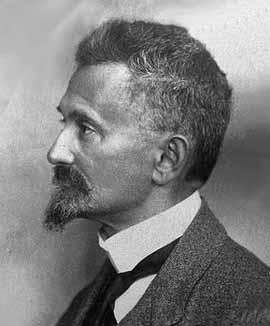
\includegraphics[width=0.4\textwidth]{felix-hausdorff.jpg}
    \caption[Felix Hausdorff,~1868--1942]{Felix Hausdorff\footnote{Převzato z~\cite{OConnorHausdorff2025}},~1868--1942}
    \label{fig:felix-hausdorff}
\end{figure}

\subsection{Definice Hausdorffovy míry}\label{subsec:hd-mira-definice}

\begin{definition}\label{def:hd-mira-delta}
    Nechť je dána množina $F\subseteq\R^n$ a $s>0$. Pak pro každé $\delta>0$ definujeme zobrazení
    \[\hausdorffdeltameasure{s}{\delta}(F)=\inf\set{\sum_{i=1}^{\infty}(\diam{F_i})^s\;\middle|\;F\subseteq\bigcup_{i=1}^\infty F_i\;,\;\diam{F_j}\leqslant\delta\;\text{pro}\;j\in\N}.\]
\end{definition}
Na první pohled si lze všimnout,~že pro $0<\delta_1<\delta_2$ je $\hausdorffdeltameasure{s}{\delta_1}(F)\geqslant\hausdorffdeltameasure{s}{\delta_2}(F)$. Jinými slovy, funkce $\delta\mapsto\hausdorffdeltameasure{s}{\delta}(M)$ je nerostoucí. Toto není nikterak těžké si rozmyslet,~neboť pro $\delta_1<\delta_2$ existuje $\delta_1$-pokrytí $\mathcal{F}_1$,~takové,~že je podpokrytím $\delta_2$-pokrytí $\mathcal{F}_2$ množiny $F$,~tedy $\mathcal{F}_1\subseteq\mathcal{F}_2$. To znamená,~že
\begin{align*}
    \hausdorffdeltameasure{s}{\delta_1}(F)&=\inf\set{\sum_{U\in\mathcal{F}_1}(\diam{U})^s\;\middle|\;\text{$\mathcal{F}_1$ je $\delta_1$-pokrytí $\mathcal{F}$}}\\
    &\geqslant\inf\set{\sum_{U\in\mathcal{F}_2}(\diam{U})^s\;\middle|\;\text{$\mathcal{F}_2$ je $\delta_2$-pokrytí $\mathcal{F}$}}=\hausdorffdeltameasure{s}{\delta_2}(F).
\end{align*}
Zároveň je z~definice \ref{def:hd-mira-delta} zjevné,~že $\mathcal{H}_\delta^s(F)\geqslant 0$.
\begin{definition}[Hausdorffova míra]\label{def:hausdorffova-mira}
    Nechť $F\subseteq\R^n$. Pak pro množinu $F$ definujeme \emph{$s$-dimenzionální Hausdorffovu míru}\index{míra!Hausdorffova} jako
    \[\hausdorffmeasure{s}(F)=\lim_{\delta\to 0}\hausdorffdeltameasure{s}{\delta}(F).\]
\end{definition}
Z přechodzího je zjevné,~že limita v~definici \ref{def:hausdorffova-mira} vždy existuje.

Bude dobré se přesvědčit,~že je Hausdorffova míra mírou ve smyslu definice \ref{def:prostor-s-mirou}. Začneme však otázkou. \emph{Na jaké množině je potřeba Hausdorffovu míru $\hausdorffmeasure{s}$ uvažovat?} Odpověď nám poskytují tzv. \emph{borelovské množiny}\index{množina!borelovská},~které jsou pojmenovány po francouzském matematikovi \name{Émile Borelovi} (1871--1956).
\begin{figure}[h]
    \centering
    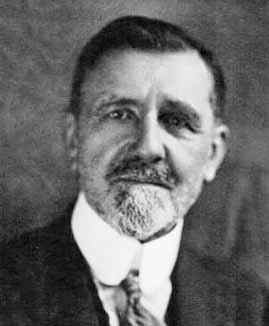
\includegraphics[width=0.4\textwidth]{Emile-Borel.jpeg}
    \caption[Émile Borel,~1871--1956]{Émile Borel\footnote{Převzato z~\cite{OConnorBorel2025}},~1871--1956}
\end{figure}
Borelovské množiny hrají podstatnou roli v~tzv. \emph{Deskriptivní teorii množin}. Nebudeme si zde vykládat všechny souvislosti,~vystačíme si se základem. Takto nazýváme všechny množiny,~které lze získat iteracemi operacemi spočetného sjednocení, průniku a doplňku otevřených množin z~$X$. Označme systém takových množin jako $\mathcal{G}$. Na tomto základě pak definujeme tzv. \emph{$\sigma$-algebru borelovských množin na $X$}:
\[\borelsigmaalgebra(X)=\bigcap_{\substack{\mathcal{F}\supseteq\mathcal{G}\\\text{$\mathcal{F}$ je $\sigma$-algebra}}}\mathcal{F}.\]
Jinými slovy,~$\borelsigmaalgebra(X)$ je nejmenší $\sigma$-algebra generovaná\footnote{Obecně $\sigma$-algebra $\mathcal{A}$ je generovaná množinou $X$,~když
\[\mathcal{A}=\bigcap_{\substack{\mathcal{F}\supseteq X\\\text{$\mathcal{F}$ je $\sigma$-algebra}}}\mathcal{F}.\]
Tento fakt se někdy značí $\mathcal{A}=\sigma(X)$.} všemi otevřenými množinami z~$X$.

Nás speciálně bude zajímat $\sigma$-algebra $\borelsigmaalgebra(\R^n)$. Nejdříve si však dokážeme dvě pomocná lemmata.
\begin{lemma}[$\sigma$-subaditivita Hausdorffovy míry]\label{lem:Hausdorffova-mira-subaditivita}
    Nechť jsou dány množiny $A_1,A_2,\ldots$,~kde $A_i\subseteq X$ pro každé $i\in\N$. Pak pro každé $s\geqslant 0$ platí
    \[\hausdorffmeasure{s}\left(\bigcup_{i=1}^\infty A_i\right)\leqslant\sum_{i=1}^{\infty}\hausdorffmeasure{s}(A_i).\]
\end{lemma}
\begin{proof}
    Nechť $s\geqslant 0$ a dále budiž dáno $\varepsilon>0$. Pro každé $i\in\N$ a $\delta>0$ mějme pokrytí
    \[\mathcal{F}_i=\set{F_{i,1},F_{i,2},\dots}\]
    množiny $A_i$,~takové,~že platí
    \[\sum_{j=1}^{\infty}(\diam{F_{i,j}})^s\leqslant\hausdorffdeltameasure{s}{\delta}(A_i)+\dfrac{\varepsilon}{2^i}.\]
    Systém $\bigcup_{i=1}^\infty\mathcal{F}_i$ tedy tvoří $\delta$-pokrytí množiny $A=\bigcup_{i=1}^\infty A_i$. Celkově
    \begin{align*}
        \hausdorffdeltameasure{s}{\delta}\left(\bigcup_{i=1}^\infty A_i\right)&\leqslant\sum_{i,j\in\N}(\diam{F_{i,j}})^s=\sum_{i=1}^{\infty}\sum_{j=1}^{\infty}(\diam{F_{i,j}})^s\leqslant\sum_{i=1}^{\infty}\left(\hausdorffdeltameasure{s}{\delta}(A_i)+\dfrac{\varepsilon}{2^i}\right)\\
        &=\sum_{i=1}^{\infty}\hausdorffdeltameasure{s}{\delta}(A_i)+\varepsilon.
    \end{align*}
    Limitním přechodem $\delta\to 0$ a aplikací Leviho věty\footnote{\emph{Leviho věta o~záměně pořadí limity a Lebesgueova integrálu} říká,~že je-li posloupnost nezáporných měřitelných funkcí $\set{f_n}_{n=1}^\infty$ neklesající,~tj.
    \[f_1\leqslant f_2\leqslant\dots\]
    na prostoru $(X,\mathcal{A},\mu)$ a zároveň $\lim_{n\to\infty}f_n(x)=f(x)$ pro každé $x\in X$,~pak
    \[\lim_{n\to\infty}\int_X f_n\dx[\mu]=\int_X \lim_{n\to\infty}f_n\dx[\mu].\]
    Zde je speciálně $\mu$ aritmetická míra, $X=\N$,~a $f_n(i)$ lze volit např. $\hausdorffdeltameasure{s}{1/n}(A_i)$. Z~Heineho věty víme,~že
    \[\lim_{n\to\infty}\hausdorffdeltameasure{s}{1/n}(A_i)=\lim_{\delta\to 0}\hausdorffdeltameasure{s}{\delta}(A_i)=\hausdorffmeasure{s}(A_i).\]
    }
    dostáváme
    \begin{align*}
        \hausdorffmeasure{s}\left(\bigcup_{i=1}^\infty A_i\right)&=\lim_{\delta\to 0}\hausdorffdeltameasure{s}{\delta}\left(\bigcup_{i=1}^\infty A_i\right)\leqslant\lim_{\delta\to 0}\sum_{i=1}^{\infty}\hausdorffdeltameasure{s}{\delta}(A_i)+\varepsilon=\sum_{i=1}^{\infty}\lim_{\delta\to 0}\hausdorffdeltameasure{s}{\delta}(A_i)+\varepsilon\\
        &=\sum_{i=1}^{\infty}\hausdorffmeasure{s}(A_i)+\varepsilon.
    \end{align*} 
\end{proof}
\begin{lemma}\label{lem:hausdorffova-mira-sigma-aditivita-kladna-vzdalenost}
    Nechť $(X,\varrho)$ je metrický prostor,~kde $X\subseteq\R^n$,~a $A,B\subseteq X$,~takové,~že pro jejich vzdálenost platí $\varrho(A,B)>0$. Pak pro každé $s\geqslant 0$ platí
    \[\hausdorffmeasure{s}(A\cup B)=\hausdorffmeasure{s}(A)+\hausdorffmeasure{s}(B).\]
\end{lemma}
\begin{proof}
    Nerovnost $\hausdorffmeasure{s}(A\cup B)\leqslant\hausdorffmeasure{s}(A)+\hausdorffmeasure{s}(B)$ je zřejmá ze $\sigma$-subaditivity Hausdorffovy míry (viz lemma \ref{lem:Hausdorffova-mira-subaditivita}).

    Bez újmy na obecnosti předpokládejme,~že $\hausdorffmeasure{s}(A\cup B)<\infty$. Mějme libovolné $\varepsilon>0$. Zvolme $\delta$-pokrytí $\mathcal{F}=\set{F_1,F_2,\ldots}$ množiny $A\cup B$,~takové,~že
    \[\sum_{i=1}^{\infty}(\diam{F_i})^s\leqslant\hausdorffdeltameasure{s}{\delta}(A\cup B)+\varepsilon.\]
    Opět bez újmy na obecnosti lze předpokládat,~že pro každé $i\in\N$ je $\diam{F_i}<\varrho(A,B)$. V~opačném případě bychom $F_i$ pokryli množnami s~menším průměrem. Z~toho pak plyne,~že každá z~množin $F_i$ má neprázdný průnik s~nejvýše jednou z~množin $A,B$,~tzn. z~pokrytí $\mathcal{F}$ lze vybrat dva disjunktní podsystémy $\mathcal{F}_A$ a~$\mathcal{F}_B$,~přičemž $\bigcup\mathcal{F}_A\supseteq A$ a $\bigcup\mathcal{F}_B\supseteq B$. Tedy celkově s~užitím předchozího lemmatu \ref{lem:Hausdorffova-mira-subaditivita} máme
    \begin{align*}
        \hausdorffdeltameasure{s}{\delta}(A)+\hausdorffdeltameasure{s}{\delta}(B)&\leqslant\hausdorffdeltameasure{s}{\delta}\left(\bigcup_{F\in\mathcal{F}_A}F\right)+\hausdorffdeltameasure{s}{\delta}\left(\bigcup_{F\in\mathcal{F}_B}F\right)\\
        &\leqslant\sum_{F\in\mathcal{F}_A}(\diam{F})^s+\sum_{F\in\mathcal{F}_B}(\diam{F})^s\\
        &\leqslant\sum_{i=1}^{\infty}(\diam{F_i})^s\leqslant\hausdorffdeltameasure{s}{\delta}(A\cup B)+\varepsilon.
    \end{align*}
    Pro $\delta\to 0$ dostáváme
    \[\hausdorffmeasure{s}(A)+\hausdorffmeasure{s}(B)\leqslant\hausdorffmeasure{s}(A\cup B)+\varepsilon\]
\end{proof}

\begin{definition}[Vnější míra]\label{def:vnejsi-mira}
    Nechť $(X,\mathcal{A})$ je měřitelný prostor. Zobrazení $\mapping{\mu^*}{\mathcal{A}}{\langle0,\infty\rangle}$ nazveme \emph{vnější mírou}\index{míra!vnější} na $\mathcal{A}$, pokud platí:
    \begin{enumerate}[label=(\alph*)]
        \item\label{def:vnejsi-mira-prazdna-mnozina} $\mu^*(\emptyset)=0$,
        \item\label{def:vnejsi-mira-monotonie} Pokud $A,B\in\mathcal{A}$ a $A\subseteq B$, pak $\mu^*(A)\leqslant\mu^*(B)$.
        \item\label{def:vnejsi-mira-sigma-subaditivita} Je-li $A_1,A_2,\ldots$ posloupnost množin, kde $A_i\in\mathcal{A}$ pro každé $i\in\N$, pak
        \[\mu^*\left(\bigcup_{i=1}^\infty A_i\right)\leqslant\sum_{i=1}^{\infty}\mu^*(A_i).\]
    \end{enumerate}
\end{definition}

Vnější míra představuje zobecnění toho, co jsme měli možnost vidět již v sekci \ref{sec:lebesgueova-mira} týkající Lebesgueovy míry\footnote{Jedná se slabší požadavek, tzn. každá míra je vnější mírou, opačné tvrzení však neplatí.}. Tu jsme definovali na základě tzv. \emph{vnější Lebesgueovy míry} (viz definice \ref{def:vnejsi-lebegueova-mira}), která sice sama o sobě míru nepředstavovala, nicméně při restrikci na "správný" systém množin jsme konstatovali, že se již jedná o míru. Lze se přesvědčit, že vnější Lebesgueova míra $\lebesgueoutermeasure{n}$ je vnější mírou ve smyslu definice \ref{def:vnejsi-mira} výše. Podobné pozorování lze učinit i pro Hausdorffovu míru $\hausdorffmeasure{s}$. Platnost podmínky \ref{def:vnejsi-mira-sigma-subaditivita} jsme dokázali v lemmatu \ref{lem:Hausdorffova-mira-subaditivita} a o platnosti \ref{def:vnejsi-mira-prazdna-mnozina} a \ref{def:vnejsi-mira-monotonie} se může čtenář velice snadno předvědčit. Tedy Hausdorffova míra na měřitelném prostoru $(X,\mathcal{A})$ je vnější mírou. Navíc pokud vnější míra $\mu^*$ splňuje závěr lemmatu \ref{lem:hausdorffova-mira-sigma-aditivita-kladna-vzdalenost}, pak ji nazýváme \emph{metrickou vnější mírou}\index{míra!metrická}\index{míra!metrická vnější}.

Carathéodoryho kritérium, které jsme si uváděli při zavádění \emph{lebesgueovské měřitelnosti}\index{měřitelnost!lebesgueovská} (viz definice \ref{def:lebesgueovska-meritelnost}). Ta jednoduše říkala, že rozdělením libovolné množiny $G$ pomocí pěvně zvolené množiny $A$ lze stanovit její míru jako součet měr dílčích částí, tzn. $G\cap A$ a $G\setminus A$. Tento koncept lze však rozšířit. Obecně jakákoliv množina je $\mu$-měřitelná, pokud splňuje Carathéodoryho kritérium.
\begin{definition}\label{def:meritelnost}
    Nechť $\mu$ je míra a $A\subseteq X$. Množina $A$ je $\mu$-měřitelná, pokud pro každé $G\subseteq X$ platí
    \[\mu(G)=\mu(G\cap A)+\mu(G\setminus A).\]
\end{definition}
Speciálně nyní ukážeme platnost následujícího tvrzení \ref{thm:hs-meritelnost-borel-mnozin}.
\begin{theorem}\label{thm:hs-meritelnost-borel-mnozin}
    Nechť $(X,\varrho)$ je metrický prostor. Pak každá množina $A\in\borelsigmaalgebra(X)$ je $\hausdorffmeasure{s}$-měřitelná pro každé $s\geqslant 0$.
\end{theorem}
\begin{proof}
    Není těžké si rozmyslet, že $\borelsigmaalgebra(X)$ vyjma otevřených množin obsahuje též všechny uzavřené\footnote{Plyne z uzavřenosti na doplněk.}. Volme tedy uzavřenou množinu $A\in\borelsigmaalgebra(X)$, $G\subseteq X$ a $s\geqslant 0$. Ze $\sigma$-subaditivity plyne nerovnost
    \[\hausdorffmeasure{s}(G)\leqslant\hausdorffmeasure{s}(G\cap A)+\hausdorffmeasure{s}(G\setminus A).\]
    Pro důkaz opačné nerovnosti definujeme posloupnost množin $P_0,P_1,P_2,\ldots$ následovně:
    \begin{align*}
        P_0&=\set{x\in G\mid\varrho(x,A)\geqslant 1},\\
        P_i&=\set{x\in G\;\middle|\;\dfrac{1}{i+1}\leqslant\varrho(x,A)\leqslant\dfrac{1}{i}}\;,\;i\geqslant 1.
    \end{align*}
    Pro libovolnou dvojici množin z podposloupnosti $P_0,P_2,P_4,\ldots$ platí, že jejich vzdálenosti jsou kladné. Z faktu, že $\hausdorffmeasure{s}$ je metrická (viz lemma \ref{lem:hausdorffova-mira-sigma-aditivita-kladna-vzdalenost}) a monotonie plyne
    \[\sum_{i=1}^{m}\hausdorffmeasure{s}(P_{2i})=\hausdorffmeasure{s}\left(\bigcup_{i=0}^m P_{2i}\right)\leqslant\hausdorffmeasure{s}(G)\]
    pro všechna $m\in\N$. Podobně pro liché členy $\sum_{i=0}^{m}\hausdorffmeasure{s}(P_{2i+1})\leqslant\hausdorffmeasure{s}(G)$. Tzn. řada $\sum_{i=0}^{\infty}\hausdorffmeasure{s}(P_i)$ je konvergentní. Zároveň platí
    \[\varrho\left(\bigcup_{i=0}^m P_i,G\cap A\right)>0,\]
    pro každé $m\in\N$, tedy lze psát
    \begin{align*}
        \hausdorffmeasure{s}(G\setminus A)&\leqslant\hausdorffmeasure{s}\left(\bigcup_{i=0}^m P_i\right)+\hausdorffmeasure{s}\left(\bigcup_{i=m+1}^\infty P_i\right)\\
        &\leqslant\hausdorffmeasure{s}(G)-\hausdorffmeasure{s}(G\cap A)+\sum_{i=m+1}^{\infty}\hausdorffmeasure{s}(P_i).
    \end{align*}
    Pro $m\to\infty$ dostáváme
    \[\hausdorffmeasure{s}(G\setminus A)\leqslant\hausdorffmeasure{s}(G)-\hausdorffmeasure{s}(G\cap A)\]
    z čehož již plyne požadovaná nerovnost.
\end{proof}
\begin{corollary}\label{cor:hausdorffova-mira-je-mira}
    Trojice $(X,\borelsigmaalgebra(X),\hausdorffmeasure{s})$,~kde $X$ je libovolná množina a $s\geqslant 0$,~tvoří prostor s~mírou.
\end{corollary}

Nyní již můžeme zobrazení $\hausdorffmeasure{s}$ nazývat mírou oprávněně. Pojďme se podívat na nějaké příklady.
\begin{example}
    Pro $s=0$ představuje zobrazení $\hausdorffmeasure{s}$ obyčejnou aritmetickou míru\index{míra!aritmetická},~tzn. pro konečnou množinu $A\subseteq\R^n$ je $\hausdorffmeasure{0}(A)=|A|$. Toto není těžké ukázat. Mějme množinu $A=\set{x_1,x_2,\ldots,x_n}$. Zvolíme-li
    \[\delta<\dfrac{1}{2}\cdot\min\set{\varrho_e(x_i,x_j)\mid 1\leqslant i,j\leqslant n},\]
    pak pro $\delta$-pokrytí $\mathcal{F}=\set{F_1,F_2,\ldots,F_n}$ takové,~že $x_i\in F_i$ pro každé $i$ máme
    \[\sum_{i=1}^{n}(\diam{F_i})^0=\sum_{i=1}^{n}1=n.\]
    Není těžké si rozmyslet,~že $n$ je nejmenší počet množin o~průměru nejvýše $\delta$,~takových,~aby pokrývaly množinu $A$. Zároveň pro libovolné $\varepsilon>0$ je potřeba nejvýše $n$-koulí o~poloměru $\varepsilon/2$ se středy v~$x_i$ pro pokrytí $A$. Tzn.~$\hausdorffmeasure{0}(A)=|A|=n$.
\end{example}

V rámci tohoto textu jsme se již zabývali jiným typem míry a to tzv. \emph{lebesgueovou mírou} (viz sekce \ref{sec:lebesgueova-mira}). Ta pro nás hrála důležitou roli v jednom možném pojetí \emph{box-counting dimenze} (viz sekce \ref{sec:box-counting-dimenze}). Lze ukázat, že pro množinu $F\subseteq\R^n$ je
\[\hausdorffmeasure{n}(F)=\dfrac{1}{v_n}\lebesguemeasure{n}(F),\]
kde $v_n$ je objem (míra) jednotkové koule v $\R^n$. Čtenář snad promine, že tento fakt zde ponecháme bez důkazu. \citep[str. 45]{Falconer2014}

\subsection{Stručně k vlastnostem Hausdorffovy míry}\label{subsec:vlastnosti-hausdorffovy-miry}

Na chvíli se ještě zastavíme u vlastností Hausdorffovy míry. Již jsme společně dokázali, že Hausdorffova míra je skutečně mírou, tzn. splňuje všechny základní vlastnosti, které jsme si představili ve větě \ref{thm:mira-vlastnosti} (viz sekce \ref{sec:prostory-s-mirou}). V tomto ohledu tedy netřeba již nic dalšího dokazovat. Nicméně podobně jako v případě \emph{box-counting dimenze} (viz podsekce \ref{subsec:vlastnosti-bc-dimenze}) se i zde podíváme, jak se Hausdorffova míra chová vůči \emph{lipschitzovským zobrazením}\index{zobrazení!lipschitzovské}.
\begin{theorem}\label{thm:hd-dimenze-lipschitzovske-zobrazeni}
    Nechť $F\subseteq\R^n$ v metrickém prostoru $(\R^n,\varrho)$ a zobrazení $\mapping{f}{F}{\R^n}$ je lipschitzovské\footnote{Tvrzení lze zformulovat obecněji pro tzv. \emph{hölderovská zobrazení}\index{zobrazení!hölderovské}, tedy zobrazení $f$ splnující
    \[\varrho(f(x),f(y))\leqslant K(\varrho(x,y))^\alpha.\]
    kde $\alpha>0$. Pak pro $F\subseteq\R^n$ platí
    \[\hausdorffmeasure{s/\alpha}(f(F))\leqslant K^{s/\alpha}\hausdorffmeasure{s}(F).\]
    My si však vystačíme se speciálním případem.} s konstantou $K>0$. Pak pro každé $s\geqslant 0$ platí
    \[\hausdorffmeasure{s}(f(F))\leqslant K^s\hausdorffmeasure{s}(F).\]
\end{theorem}
\begin{proof}
    Nechť $\mathcal{F}=\set{F_1,F_2,\ldots}$ je $\delta$-pokrytí $F$. Pak
    \[\diam(f(F\cap F_i))\leqslant K\diam(F\cap F_i)\leqslant K\diam{F_i},\]
    což znamená, že $\mathcal{G}=\set{F\cap F_1,F\cap F_2,\ldots}$ je $K\delta$-pokrytí $f(F)$. Z toho plyne, že
    \[\sum_{i=1}^{\infty}(\diam(f(F\cap F_i)))^s\leqslant K^s\sum_{i=1}^{\infty}(\diam{F_i})^s\]
    a tedy $\hausdorffdeltameasure{s}{K\delta}(f(F))\leqslant K^s\hausdorffdeltameasure{s}{\delta}(F)$. Pro $\delta\to 0$ máme požadovaný výsledek.
\end{proof}
(Převzato z \citep[str. 46]{Falconer2014}.)

Z toho speciálně plyne důsledek týkající se podobností.
\begin{corollary}\label{cor:hd-dimenze-podobnost}
    Nechť $F\subseteq\R^n$ v metrickém prostoru $(\R^n,\varrho)$ a zobrazení $\mapping{f}{F}{\R^n}$ je podobnost\index{podobnost}, tzn. existuje $K>0$ takové, že pro každé $x,y\in F$ platí
    \[\varrho(f(x),f(y))=K\varrho(x,y).\]
    Pak pro každé $s\geqslant 0$ platí
    \[\hausdorffmeasure{s}(f(F))=K^s\hausdorffmeasure{s}(F).\]
\end{corollary}
\begin{proof}
    K podobnosti $f$ existuje inverzní zobrazení $f^{-1}$ s koeficientem $L=1/K$. Z věty \ref{thm:hd-dimenze-lipschitzovske-zobrazeni} tedy plyne, že
    \[\hausdorffmeasure{s}(F)=\hausdorffmeasure{s}(f^{-1}(f(F)))\leqslant\dfrac{1}{K^s}\hausdorffmeasure{s}(f(F))\]
    nebo-li $\hausdorffmeasure{s}(f(F))\geqslant K^s\hausdorffmeasure{s}(F)$. Opačnou nerovnost získáme aplikací věty \ref{thm:hd-dimenze-lipschitzovske-zobrazeni} na zobrazení $f$.
\end{proof}

\subsection{Hausdorffova dimenze}\label{subsec:hausdorffova-dimenze}

Středobodem této sekce je tzv. \emph{Hausdorffova dimenze}\index{dimenze!Hausdorffova}. Na úvod si dokážeme jedno jednoduché tvrzení týkající se Hausdorffovy míry.
\begin{theorem}\label{thm:hodnoty-hausdorffovy-miry}
    Nechť $0\leqslant s<t<\infty$ a $F\subseteq X$. Pak platí:
    \begin{enumerate}[label=(\roman*)]
        \item\label{thm:hd-dimenze-konecna} $\hausdorffmeasure{s}(F)<\infty\implies\hausdorffmeasure{t}(F)=0$,
        \item\label{thm:hd-dimenze-nekonecno} $\hausdorffmeasure{t}(F)>0\implies\hausdorffmeasure{s}(F)=\infty$.
    \end{enumerate}
\end{theorem}
\begin{proof}
    Mějme $\delta$-pokrytí $\mathcal{F}=\set{F_1,F_2,\ldots}$,~takové,~že
    \[\sum_{i=1}^{\infty}(\diam{F_i})^s\leqslant\hausdorffdeltameasure{s}{\delta}(F)+\varepsilon\;,\;\varepsilon>0.\]
    Pak
    \[\hausdorffdeltameasure{t}{\delta}(F)\leqslant\sum_{i=1}^{\infty}(\diam{F_i})^t\leqslant\delta^{t-s}\sum_{i=1}^{\infty}(\diam{F_i})^s\leqslant\delta^{t-s}(\hausdorffdeltameasure{s}{\delta}(F)+\varepsilon).\]
    Tzn.~$\hausdorffdeltameasure{t}{\delta}(F)\leqslant\delta^{t-s}\hausdorffdeltameasure{s}{\delta}(F)$. Pro $\delta\to 0$ dostaneme body \ref{thm:hd-dimenze-konecna} a \ref{thm:hd-dimenze-nekonecno}.
\end{proof}
(Převzato z~\citep[str. 68]{Mattila1995}.)

Z věty \ref{thm:hodnoty-hausdorffovy-miry} lze vidět,~že Hausdorffova míra dává smysl jen pro určitou hodnotu $s$. Pro "příliš velké" $s$ bude hodnota vždy $0$,~naopak pro "moc malé" $s$ bude jeho hodnota rovna $\infty$ (viz obrázek \ref{fig:hausdorffova-dimenze-graf}).
\begin{figure}[h]
    \centering
    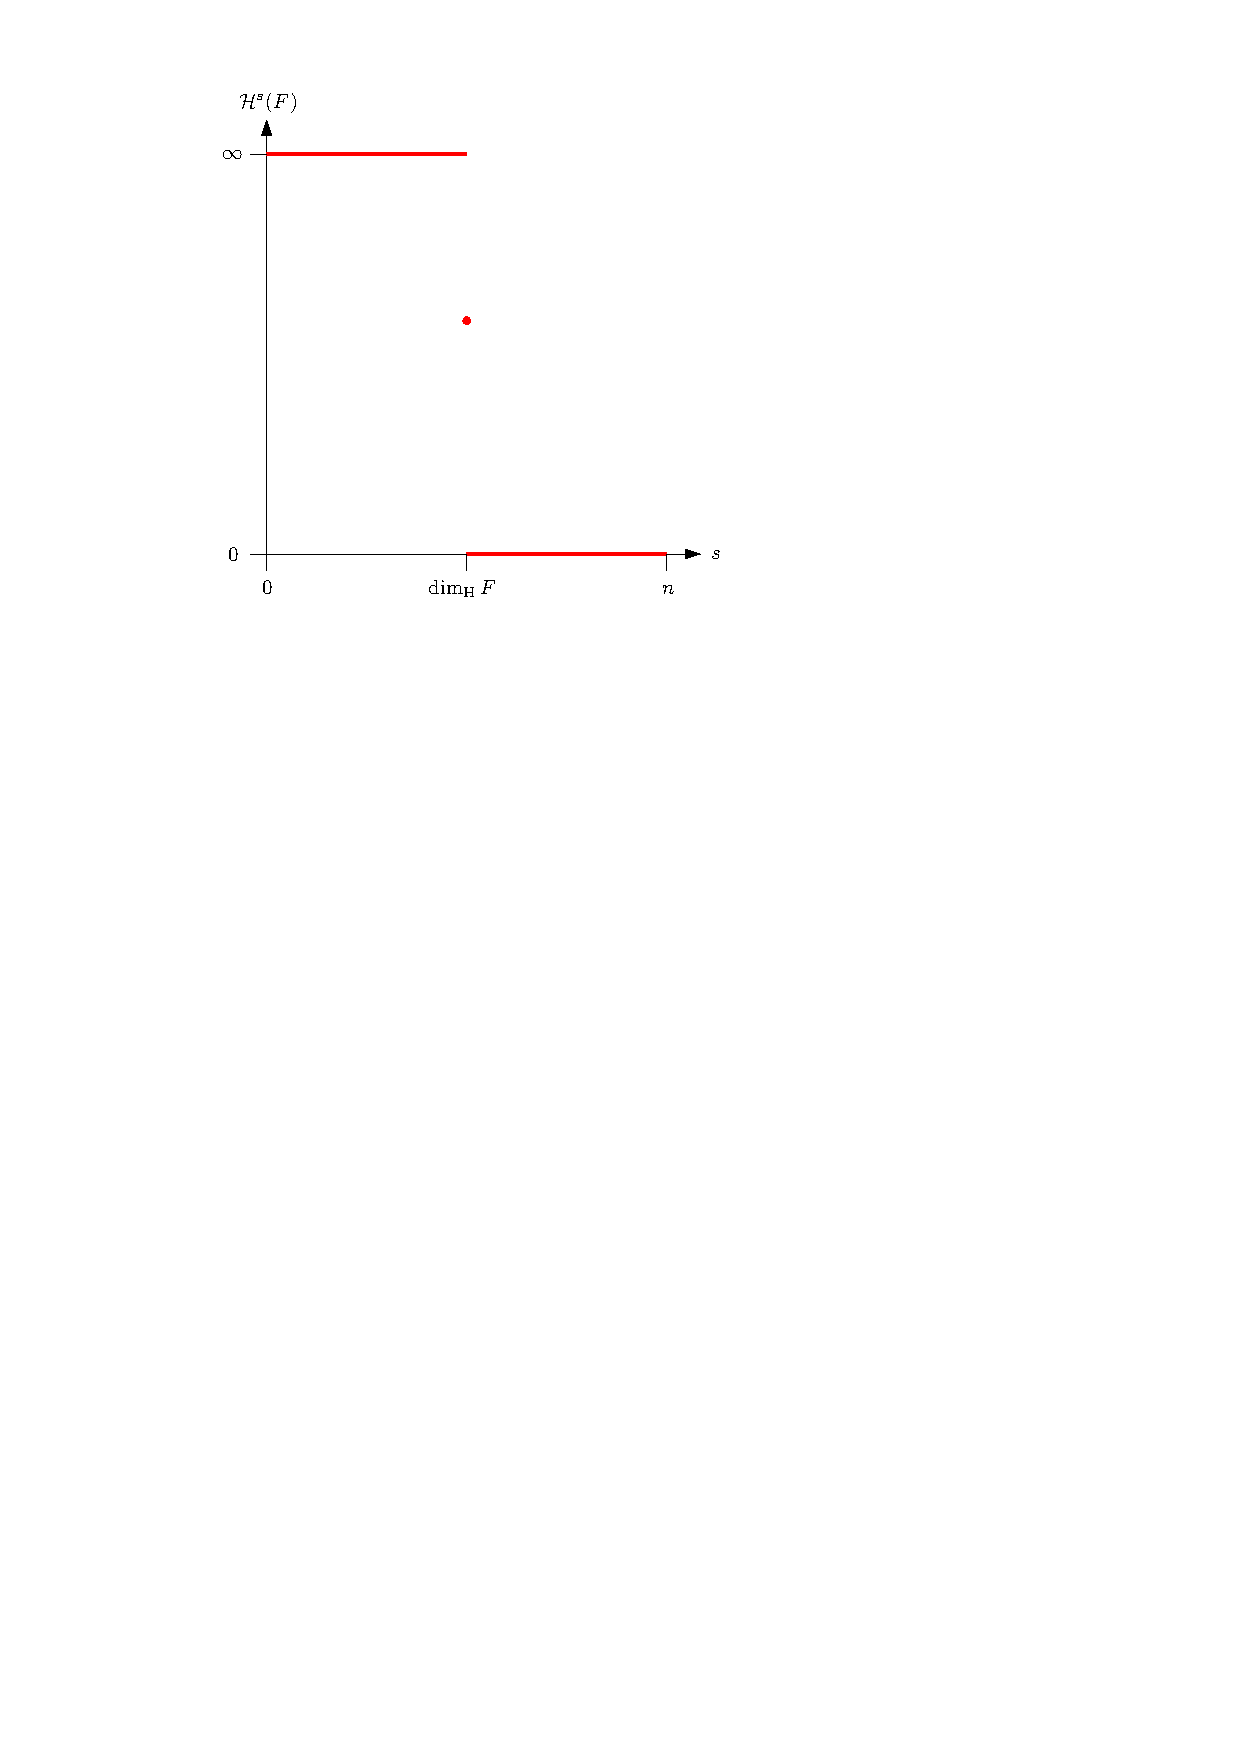
\includegraphics{ch02-hausdorffova-dimenze-graf.pdf}
    \caption{Graf funkce $f(s)=\hausdorffmeasure{s}(F)$,~kde $F\subseteq\R^n$.}
    \label{fig:hausdorffova-dimenze-graf}
\end{figure}
Této kritické hodnotě $s$ říkáme \emph{Hausdorffova dimenze}\index{dimenze!Hausdorffova}.
\begin{definition}[Hausdorffova dimenze]\label{def:hausdorffova-dimenze}
    Nechť $F\subseteq\R^n$. Hausdorffovou dimenzí\footnote{Též někdy nazývaná \emph{Hausdorffova-Bezikovičova dimenze}\index{dimenze!Hausdorffova-Bezikovičkova}. }\index{dimenze!Hausdorffova} množiny $F$ nazveme hodnotu
    \[\dimH{F}=\inf\set{s\geqslant 0\mid\hausdorffmeasure{s}(F)=0}=\sup\set{s\geqslant 0\mid\hausdorffmeasure{s}(F)=\infty}.\]
\end{definition}
Hodnota $\hausdorffmeasure{s}(F)$ pro $s=\dimH{F}$ může být různá,~tzn. může platit,~že $\hausdorffmeasure{s}(F)=\infty$,~$\hausdorffmeasure{s}(F)=0$ a nebo se může jednat o~konečné nenulové číslo,~tj. $0<\hausdorffmeasure{s}(F)<\infty$.

Nyní se podívejme na příklad výpočtu. Podobně, jako v případě box-counting dimenze, i zde budeme nezávisle určovat horní a dolní odhad.
\begin{example}[Sierpińského trojúhelník]\label{ex:sierpinskeho-trojuhelnik-hd-dimenze}
    V tomto případě se podíváme na dvě možnosti, jak dojít k výsledku. Celý Sierpińského trojúhelník si označme $S$.
    \begin{itemize}
        \item V $k$-té iteraci, kde $k=0,1,2,\ldots$, vzniknou 3 nové trojúhelníky o obsahu $1/4$ obsahu původního trojúhelníka, tzn. jejich celkový počet je $t=3^k$. Uvažíme-li $\delta$-pokrytí
        \[\mathcal{K}=\set{K_\delta^1(x_1),K_\delta^2(x_2),\ldots,K_\delta^t(x_t),\emptyset,\emptyset,\ldots}\]
        kde $x_1,x_2,\ldots,x_t\in S_k$ a $\delta\leqslant 2^{-k}/2=2^{-k-1}$, pak
        \[\hausdorffdeltameasure{s}{2^{-k}}(S_k)\leqslant\sum_{i=1}^{3^k}(2^{-k})^s=3^k2^{-ks}=1.\]
        Pro $k\to\infty$ je $\hausdorffmeasure{s}(S)\leqslant 1$. Poslední rovnost nastává právě pro $s=\ln{3}/\ln{2}$.

        Nyní ukážeme, že $\hausdorffmeasure{s}(S)\geqslant 3^{-s}=1/2$. Zvolme $\delta$-pokrytí $\mathcal{F}=\set{F_1,F_2,\ldots}$, takové, že
        \begin{equation}\label{eq:volba-delta-pokryti-F}
            2^{-k-1}\leqslant\diam{F_i}<2^{-k},
        \end{equation}
        kde $i\in\N$. Lze si rozmyslet, že každá z množin $F_i$ má neprázdný průnik s nejvýše dvěma dílčími trojúhelníky. Zvolíme-li $j\geqslant k$, pak každá z množin $F_i$ má průnik maximálně s $3^{j-k}$ trojúhelníky v $j$-té iteraci, resp.
        \[3^{j-k}=3^j2^{-ks}\leqslant2^j3^s(\diam{F_i})^s,\]
        jak plyne z volby pokrytí $\mathcal{F}$ v \eqref{eq:volba-delta-pokryti-F}. Pokud navíc pro každé $i\in\N$ platí, že
        \[3^{-j-1}\leqslant\diam{F_i},\]
        pak každá z množin $F_i$ má neprázdný průnik s nejvýše $3^j$ trojúhelníky. Tedy pro jejich počet platí
        \[3^j\leqslant\sum_{i=1}^{\infty}3^j3^s(\diam{F_i})^s,\]
        přičemž úpravou už získáme požadovanou nerovnost.
        \item Druhá varianta výpočtu je sice méně rigorózní, avšak podstatně jednodušší. Sierpińského trojúhelník sestává ze tří kopií sebe samotného, přičemž každá z nich je obrazem původního obrazce $S$ v podobnosti s koeficientem $K=1/2$. Označme si dané části $S_1,S_2$ a $S_3$, tj. $S=S_1\cup S_2\cup S_3$. Tedy podle $\sigma$-aditivity Hausdorffovy míry a důsledku \ref{cor:hd-dimenze-podobnost} můžeme psát
        \begin{align*}
            \hausdorffmeasure{s}(S)&=\hausdorffmeasure{s}(S_1)+\hausdorffmeasure{s}(S_2)+\hausdorffmeasure{s}(S_3)\\
            &=\left(\dfrac{1}{2}\right)^s\hausdorffmeasure{s}(S)+\left(\dfrac{1}{2}\right)^s\hausdorffmeasure{s}(S)+\left(\dfrac{1}{2}\right)^s\hausdorffmeasure{s}(S)\\
            &=3\left(\dfrac{1}{2}\right)^s\hausdorffmeasure{s}(S).
        \end{align*}
        Budeme-li předpokládat, že $\hausdorffmeasure{s}(S)<\infty$ (jak jsme již viděli z předchozího výpočtu, jedná se o netriviální předpoklad) pro $s=\dimH{S}$, pak z rovnosti $1=3(1/2)^s$ lze dopočítat, že $s=\ln{3}/\ln{2}$.
    \end{itemize}
\end{example}
(Převzato a upraveno z \citep[str. 53]{Falconer2014}.)

Myšlenku druhého výpočtu z příkladu \ref{ex:sierpinskeho-trojuhelnik-hd-dimenze} ještě rozvedeme v kapitole \ref{chapter:klasifikace-fraktalu}, konkrétně v sekci \ref{sec:ifs} věnované systémům iterovaných funkcí\index{systém iterovaných funkcí}.

Jako poslední zkusme postavit Hausdorffovu dimenzi proti box-counting dimenzi, kterou jsme si představili v sekci \ref{sec:box-counting-dimenze}. 